\documentclass[conference]{IEEEtran}

\usepackage{amsmath}
\usepackage{amssymb}
\usepackage{graphicx}
\setlength{\tabcolsep}{4pt}
\setlength{\abovedisplayskip}{8pt}
\setlength{\belowdisplayskip}{8pt}
\newtheorem{proposition}{Proposition}
% hyperref omitted (not available in this build environment)

% Custom algorithm environment (algorithm/algpseudocode not available)
\newcounter{algorithm}
\newcounter{algorithmlinenum}
\newenvironment{algorithm}[1][]
  {\setcounter{algorithmlinenum}{0}\refstepcounter{algorithm}\par\medskip\noindent\textbf{Algorithm~\thealgorithm: #1}\par\smallskip\begin{quote}}
  {\end{quote}\par\medskip}
\newcommand{\algorithminput}[1]{\textbf{Input:} #1\\}
\newcommand{\algorithmoutput}[1]{\textbf{Output:} #1\\}
\newcommand{\algorithmstep}[1]{\stepcounter{algorithmlinenum}\hspace*{1em}\thealgorithmlinenum.~#1\\}
\newcommand{\algorithmfor}[1]{\stepcounter{algorithmlinenum}\hspace*{1em}\thealgorithmlinenum.~\textbf{for} #1 \textbf{do}\\}
\newcommand{\algorithmendfor}{\stepcounter{algorithmlinenum}\hspace*{1em}\thealgorithmlinenum.~\textbf{end for}\\}
\newcommand{\algorithmif}[1]{\stepcounter{algorithmlinenum}\hspace*{1em}\thealgorithmlinenum.~\textbf{if} #1 \textbf{then}\\}
\newcommand{\algorithmelse}{\stepcounter{algorithmlinenum}\hspace*{1em}\thealgorithmlinenum.~\textbf{else}\\}
\newcommand{\algorithmendif}{\stepcounter{algorithmlinenum}\hspace*{1em}\thealgorithmlinenum.~\textbf{end if}\\}
\newcommand{\algorithmreturn}[1]{\stepcounter{algorithmlinenum}\hspace*{1em}\thealgorithmlinenum.~\textbf{return} #1\\}

\pdfinfo{
  /Title (Interaction Impact Score: Evaluating the Predictive Utility of Statistically Significant Feature Interactions in Workforce Analytics)
  /Author (Nayan Dhurve)
  /Subject (Workforce Analytics, Interaction Mining, Predictive Modeling)
  /Keywords (Workforce Analytics; Interaction Mining; Feature Interactions; HR Analytics; Predictive Modeling; SHAP; XGBoost; Explainable AI)
}

\title{Interaction Impact Score: Evaluating the Predictive Utility of Statistically Significant Feature Interactions in Workforce Analytics}

\author{
    \IEEEauthorblockN{Nayan Dhurve}
    \IEEEauthorblockA{
        Independent Researcher\\
        Nagpur, Maharashtra, India\\
        \texttt{nayankdhurve@gmail.com}\\
        ORCID: 0009-0005-8051-4988
    }
}

\begin{document}

\maketitle

\begin{abstract}
Feature interactions are widely recognized as important in machine learning, yet their practical utility in workforce analytics remains unclear. This paper investigates whether statistically significant feature interactions improve predictive performance or serve primarily interpretive purposes. We introduce an Interaction Impact Score as a measurement instrument---combining mutual information, outcome differential, and segment size---and evaluate it through exhaustive pairwise interaction mining (1,755 pairs, five outcomes, three model families). Our findings reveal a nuanced picture: strong, statistically significant interactions exist (the strongest achieves impact 181.3) and follow a heavy-tailed Pareto distribution (3.1\% of pairs drive 80\% of total impact). However, adding interaction features as explicit predictors does not provide statistically significant accuracy improvements---the mean change is $+0.008\pm0.021$ (range $-0.038$ to $+0.044$), and no configuration passes the Wilcoxon signed-rank test ($p < 0.05$). The effects are inconsistent: Logistic Regression shows both the largest improvements and the largest degradation, while tree-based models are essentially unchanged. We conclude that the primary value of interaction mining in workforce analytics lies in \textit{interpretability} rather than predictive gains. External validation across 5 datasets spanning 4 domains (synthetic HR, IBM HR, Adult Census, Bank Marketing, Telco Churn) shows consistent patterns.
\end{abstract}

\begin{IEEEkeywords}
Workforce Analytics, Interaction Mining, Feature Interactions, HR Analytics, Predictive Modeling, SHAP, XGBoost, Explainable AI
\end{IEEEkeywords}

% ============================================================================
\section{Introduction}
\label{sec:introduction}
% ============================================================================

Human resource decisions fundamentally shape organizational success. Yet traditional practices rely heavily on interview-based assessment, which is susceptible to systematic biases including extroversion preference, cultural norm alignment, and confirmation bias \cite{fabris2025fairness}. An introverted but technically brilliant candidate may be overlooked in a culture that rewards self-promotion, while an outspoken candidate may be seen as disruptive in a culture that values group harmony.

Data-driven workforce analytics offers a path beyond these limitations. By systematically analyzing the rich data that organizations already collect---demographics, performance ratings, tenure patterns, compensation structures, career trajectories---we can develop a more complete, less biased understanding of employees.

Most existing work in HR analytics focuses on predicting a single outcome, most commonly employee attrition \cite{talebi2025systematic}. While valuable, this narrow focus misses the multi-dimensional nature of workforce dynamics and, critically, ignores the role of \textit{interaction effects}: combinations of features often matter more than individual features alone. For example, tenure may relate to performance differently for managers than for individual contributors; compensation equity may manifest differently across departments and demographic groups.

This paper addresses these gaps by investigating four research questions:

\begin{enumerate}
    \item[RQ1] Which pairwise feature interactions exhibit statistically significant associations with workforce outcomes?
    \item[RQ2] Do statistically significant interactions improve predictive performance when added as explicit features?
    \item[RQ3] How consistent are interaction rankings across independent datasets?
    \item[RQ4] Can interaction mining provide organizational insights independent of predictive gains?
\end{enumerate}

\subsubsection*{Contributions}
This work makes the following contributions:
\begin{enumerate}
    \item \textit{Exhaustive interaction scan:} Systematic testing of all 1,755 pairwise feature combinations across five workforce outcomes and three model families, providing the first comprehensive interaction map in HR analytics.
    \item \textit{Negative-result ablation:} Rigorous with/without interaction feature comparison using paired statistical tests (Wilcoxon and paired t-test), indicating that explicit interaction engineering provides no measurable predictive benefit for tree-based models.
    \item \textit{Paradox identification:} Discovery and explanation of the PayZone paradox---the strongest interaction yet near-random prediction---and class-imbalance model-family behavior, providing methodological guidance for practitioners.
    \item \textit{Practical recommendations:} A decision framework for when interaction mining adds value (exploratory analysis, policy evaluation, hypothesis generation) versus when it does not (predictive optimization with tree ensembles).
\end{enumerate}

\subsubsection*{Hypothesis}
We test the hypothesis that statistically significant pairwise feature interactions, when encoded as explicit features, improve predictive performance across multiple workforce prediction tasks compared to models using only main effects. This hypothesis is evaluated across five outcomes, three model families, and five datasets.

To answer these questions, we introduce an Interaction Impact Score as a measurement instrument---combining mutual information, outcome differential, and segment size---and apply it within a systematic seven-phase pipeline. Our findings indicate that while the Interaction Impact Score identifies strong, statistically significant interactions---particularly JobFamily $\times$ DepartmentType and Tenure $\times$ Exit Quarter (impact scores exceeding 100)---adding these interactions as explicit features yields no statistically significant improvement in predictive accuracy. This reveals that the value of interaction mining lies in \textit{interpretability and hypothesis generation} rather than raw predictive gains.

The remainder of this paper is organized as follows: Section~\ref{sec:related} discusses related work. Section~\ref{sec:methodology} describes our dataset, pipeline, and methodology. Section~\ref{sec:results} presents experimental results. Section~\ref{sec:discussion} discusses implications and limitations. Section~\ref{sec:conclusion} concludes and outlines future directions.

% ============================================================================
\section{Related Work}
\label{sec:related}
% ============================================================================

\subsection{HR Analytics and Predictive Modeling}

The field of HR analytics has grown substantially, with employee attrition prediction being the dominant research focus. Talebi et al. \cite{talebi2025systematic} conducted a systematic review of 62 studies and found that Random Forest is the most frequently used model, job satisfaction is the single most predictive feature, and the IBM HR dataset \cite{ibmhr} is the most commonly used benchmark. Most studies report accuracy in the 70--90\% range depending on dataset and methodology. De Vos et al. \cite{devos2024predicting} reached similar conclusions, noting that ensemble methods consistently outperform single classifiers for attrition prediction. Alduayj and Rajpoot \cite{alduayj2020predicting} showed that gradient boosting achieves the highest accuracy (87\%) on the IBM dataset, though at the cost of interpretability.

Alyousef et al. \cite{alyousef2026hybrid} proposed a hybrid predictive model for employee turnover using XGBoost with SHAP (SHapley Additive exPlanations) interpretability, identifying interaction between job level and experience as a key attrition driver. However, like most work in this area, they used SHAP's built-in interaction detection post-hoc rather than systematic pre-model interaction testing. Al Akasheh et al. \cite{alakasheh2023decade} extended this by incorporating temporal features and found that tenure-interaction terms improve attrition prediction by 2--4\%, consistent with the effect sizes we observe in our study.

\subsection{Interaction Effects in Machine Learning}

Feature interactions are recognized as important across many domains. Friedman and Popescu \cite{friedman2008predictive} introduced the H-statistic, a model-agnostic measure that decomposes prediction variance into main and interaction effects. Lou et al. \cite{lou2013accurate} developed GA$^2$M, which explicitly models pairwise interactions within a Generalized Additive Model framework, achieving both accuracy and intelligibility. Caruana et al. \cite{caruana2015intelligible} showed the practical value of interaction-aware models in healthcare, where pairwise interactions improved pneumonia risk prediction.

Tree-based models naturally capture interactions through their hierarchical splitting structure. Breiman's Random Forest \cite{breiman2001random} and Chen and Guestrin's XGBoost \cite{chen2016xgboost} implicitly model interactions without explicit feature engineering. However, Sorokina et al. \cite{sorokina2008detecting} showed that tree ensembles can reliably detect additive interactions when explicitly tested, motivating systematic interaction search strategies. Lundberg and Lee \cite{lundberg2017unified} extended their SHAP framework to pairwise interaction values \cite{lundberg2020shap}, enabling post-hoc interaction detection within tree-based models. Tsang et al. \cite{tsang2018detecting} introduced neural interaction detection (NID), which extracts interaction effects from trained neural networks.

\subsection{Why Existing Interaction Detection Methods Are Insufficient}

Existing methods for detecting feature interactions each address a subset of desiderata, but no single method satisfies all requirements for systematic pre-model interaction mining. We identify five criteria essential for this task: (C1) model-agnostic---computable before any model training; (C2) nonlinear---detecting non-product-moment dependencies; (C3) quantitative---producing a ranked impact metric, not just a significance decision; (C4) multi-outcome---scalable across prediction targets; (C5) significance-aware---with built-in statistical testing. We evaluate existing methods against these criteria in Table~\ref{tab:method_comparison}.

\begin{table}[htb]
\centering
\small
\renewcommand{\arraystretch}{1.15}
\caption{Comparison of interaction detection methods across five criteria for systematic pre-model mining.}
\label{tab:method_comparison}
\begin{tabular}{lccccc}
\hline
Method & Free & Nonlin. & Metric & Multi & Sig. \\
\hline
Pearson corr. & Yes & No & No & Yes & Yes \\
Mutual Info. & Yes & Yes & No & Yes & No \\
$\chi^2$ test & Yes & Yes & No & Yes & Yes \\
Additive Groves \cite{sorokina2008detecting} & Yes & Yes & No & Part. & Yes \\
SHAP inter. \cite{lundberg2020shap} & No & Yes & Yes & Dep. & No \\
H-statistic \cite{friedman2008predictive} & Yes & Yes & Yes & No & No \\
Impact Score & Yes & Yes & Yes & Yes & Yes \\
\hline
\end{tabular}
\end{table}

\noindent\textbf{Pearson correlation} detects only linear (product-moment) dependencies. Workforce interactions---e.g., JobFamily $\times$ DepartmentType predicting PayZone---are inherently categorical and nonlinear, making Pearson incapable of detecting the strongest signals we discover.

\textbf{Mutual Information (MI)} captures nonlinear dependence but provides no ranking metric beyond the raw MI value, which conflates dependence strength with feature entropy and lacks any sample-size penalty. MI alone places TenureYears $\times$ TenureVsAvg (MI=4.30) above JobFamily $\times$ DepartmentType (MI=0.60) in our data, despite the latter having far greater practical significance.

\textbf{$\chi^2$ and ANOVA tests} provide significance decisions but no unified impact metric. A $\chi^2$ of 1423 (our top-ranked pair) and 1000 (our third-ranked pair) are both astronomically significant ($p<10^{-100}$), yet the test statistic alone cannot distinguish which interaction has greater practical impact. The Impact Score resolves this by weighting significance by outcome differential and segment size.

\textbf{SHAP interaction values} are model-specific by construction---they require a trained model and reflect prediction decomposition rather than population-level association. In our comparison, SHAP and the Impact Score show no significant rank correlation (Spearman $\rho=-0.140$, $p=0.126$), confirming that SHAP emphasizes model-internal dynamics (e.g., TenureDays $\times$ TenureVsAvg as the top SHAP pair) while the Impact Score captures broader cross-feature associations. SHAP also scales poorly: computing SHAP interaction values for all 1,755 pairs across 3 models is computationally prohibitive.

\textbf{The H-statistic} is model-agnostic but computationally expensive ($O(N\cdot p^2\cdot B)$ with $B$ bootstrap iterations) and provides per-pair rather than per-outcome rankings. Computing H for all 1,755 pairs against 5 outcomes is impractical.

\subsection{The Gap: Systematic Interaction Mining in HR}

While interaction detection methods are well-established in the ML literature, their application in HR analytics has been piecemeal. Most papers either ignore interactions entirely or rely on model-specific post-hoc detection (e.g., SHAP interaction values from a single XGBoost model). No existing work performs an \textit{exhaustive systematic scan} of all pairwise interactions across multiple outcomes and models, which is the gap our paper addresses. Furthermore, existing studies typically examine a single outcome (most often attrition), missing the multi-outcome nature of workforce dynamics. This leaves open the central question we investigate: whether statistically significant interactions in workforce data translate into predictive utility or serve primarily interpretive purposes.

\subsection{Fairness and Bias in HR Analytics}

A growing body of work examines fairness and bias in algorithmic HR systems. Fabris et al. \cite{fabris2025fairness} provide a comprehensive survey of bias in algorithmic hiring, covering bias sources, detection methods, and mitigation strategies. Sony et al. \cite{sony2025bias} examine discrimination risks embedded in AI-driven HR tools, identifying three high-risk categories: data bias (skewed training data), algorithmic bias (model architecture choices), and deployment bias (misapplication of predictions). Wingate et al. \cite{wingate2024bias} identify six high-risk applicant characteristics that introduce bias into employment interviews, including extroversion preference, cultural similarity, and physical attractiveness.

Mehrabi et al. \cite{mehrabi2021survey} provide a comprehensive taxonomy of bias sources in machine learning pipelines, distinguishing between data-driven, algorithmic, and human-induced biases. Hardt et al. \cite{hardt2016equality} formalized equality of opportunity as a fairness metric, which is particularly relevant for HR applications where false positives (incorrectly flagging an employee as high-risk) and false negatives carry different costs.

Our work connects to this literature by showing how data-driven capability assessment---grounded in systematic interaction mining---can reduce reliance on interview-only evaluation, potentially mitigating bias. We further discuss ethical safeguards in Section~\ref{sec:discussion}. In summary, existing work has established the value of feature interactions in specific ML contexts but has not provided a generalizable, task-agnostic framework for discovering high-impact interactions in workforce data across multiple outcomes.

% ============================================================================
\section{Methodology}
\label{sec:methodology}
% ============================================================================

\subsection{Dataset}

We evaluate the Interaction Impact Score across 5 datasets spanning 4 domains (Table~\ref{tab:datasets}). The primary analysis uses a synthetic workforce dataset of 3,000 employee records with 26 raw columns covering demographics, employment history, job characteristics, performance, and termination details. The data is synthetic---a transparent limitation that ensures reproducibility and avoids privacy concerns while providing control over ground-truth interaction structure. We mitigate this through cross-domain validation on 4 additional public datasets: IBM HR Attrition (Kaggle, 1,470 records), Adult Census Income (UCI, 32,561 records), Bank Marketing (UCI, 45,211 records), and Telco Customer Churn (Kaggle, 7,043 records).

From the 26 raw columns, we engineer 27 features for interaction mining during Phase 2 of our pipeline. The feature categories are listed in Table~\ref{tab:features}. The evaluation datasets are summarized in Table~\ref{tab:datasets}.

\begin{table}[htb]
\centering
\footnotesize
\renewcommand{\arraystretch}{1.15}
\caption{Datasets used for cross-domain validation.}
\label{tab:datasets}
\begin{tabular}{llrr}
\hline
Dataset & Domain & Rows & Source \\
\hline
Synthetic Workforce & HR & 3,000 & Simulated \\
IBM HR Attrition & HR & 1,470 & Kaggle \\
Adult Census Income & Census & 32,561 & UCI \\
Bank Marketing & Banking & 45,211 & UCI \\
Telco Customer Churn & Telecom & 7,043 & Kaggle \\
\hline
\end{tabular}
\end{table}

\begin{table}[htb]
\centering
\footnotesize
\renewcommand{\arraystretch}{1.15}
\caption{Feature categories and counts used in interaction mining.}
\label{tab:features}
\begin{tabular}{lrp{2.8cm}}
\hline
Category & Count & Examples \\
\hline
Demographics & 5 & Age, CareerStage, Generation, GenderCode, RaceDesc \\
Tenure \& Employment & 4 & TenureYears, TenureDays, TenureVsAvg, IsLongTenure \\
Role \& Hierarchy & 10 & JobFamily, SeniorityLevel, DepartmentType, IsManager \\
Compensation \& Diversity & 3 & IntersectionalID, DeptDiversityScore, DeptGenderRatio \\
Temporal & 4 & StartYear, StartQuarter, ExitYear, ExitQuarter \\
Performance & 1 & PerfScore \\
\hline
\end{tabular}
\end{table}

The categories described in Table~\ref{tab:features} form the basis of our analysis targeting five outcome variables spanning workforce dynamics:

\begin{itemize}
    \item \textit{is\_terminated} (binary): whether the employee's status contains ``Terminated''
    \item \textit{PayZone} (3-class): compensation zone assignment (Zone A/B/C)
    \item \textit{is\_minority\_dept} (binary): for each department, whether the employee's gender is the minority gender in that department
    \item \textit{PerfScore} (multiclass): current employee performance rating
    \item \textit{SeniorityLevel} (multiclass): derived career seniority score from the feature engineering phase
\end{itemize}

Of these, is\_terminated and is\_minority\_dept are binary outcomes for which Area Under the ROC Curve (AUC) can be reported; PayZone is a 3-class ordinal target; and PerfScore and SeniorityLevel are engineered features. Target leakage pathways for all outcomes are explicitly identified and excluded (see Section~\ref{sec:leakage}).

\subsection{Target Leakage Prevention}
\label{sec:leakage}

A critical methodological concern in interaction mining pipelines is target leakage---when the feature matrix inadvertently contains information derived from the target variable. During initial development, we identified three leakage pathways that produced artificially inflated accuracy:

\begin{itemize}
    \item \textit{PerfScore self-prediction:} When predicting PerfScore, the PerfScore column itself was included as a feature, producing 99.9\% accuracy. The fix excludes the target column from the feature matrix when its name matches a feature column.
    \item \textit{SeniorityLevel derived features:} The columns IsExecutive and IsIC are deterministically derived from SeniorityLevel, creating an indirect leakage pathway. The fix excludes all three (SeniorityLevel, IsExecutive, IsIC) when predicting SeniorityLevel.
    \item \textit{Termination post-hoc columns:} ExitYear and ExitQuarter partially encode termination status (active employees have missing exit dates). The fix excludes these columns when predicting is\_terminated.
\end{itemize}

All results in this paper reflect the corrected pipeline. The most impacted outcomes are PerfScore (accuracy dropped from 0.999 to 0.739) and SeniorityLevel (1.000 to 0.946), while termination and minority-department predictions changed negligibly (${<}0.01$), indicating these were genuine leakage effects rather than general pipeline errors. This correction is documented in the reproducibility checklist and enforced by a \texttt{\_LEAKAGE\_EXCLUDE} dictionary in the open-source codebase.

\subsection{Seven-Phase Pipeline}

Our analysis follows a seven-phase pipeline (Figure~\ref{fig:pipeline}):

\begin{figure*}[t]
\centering
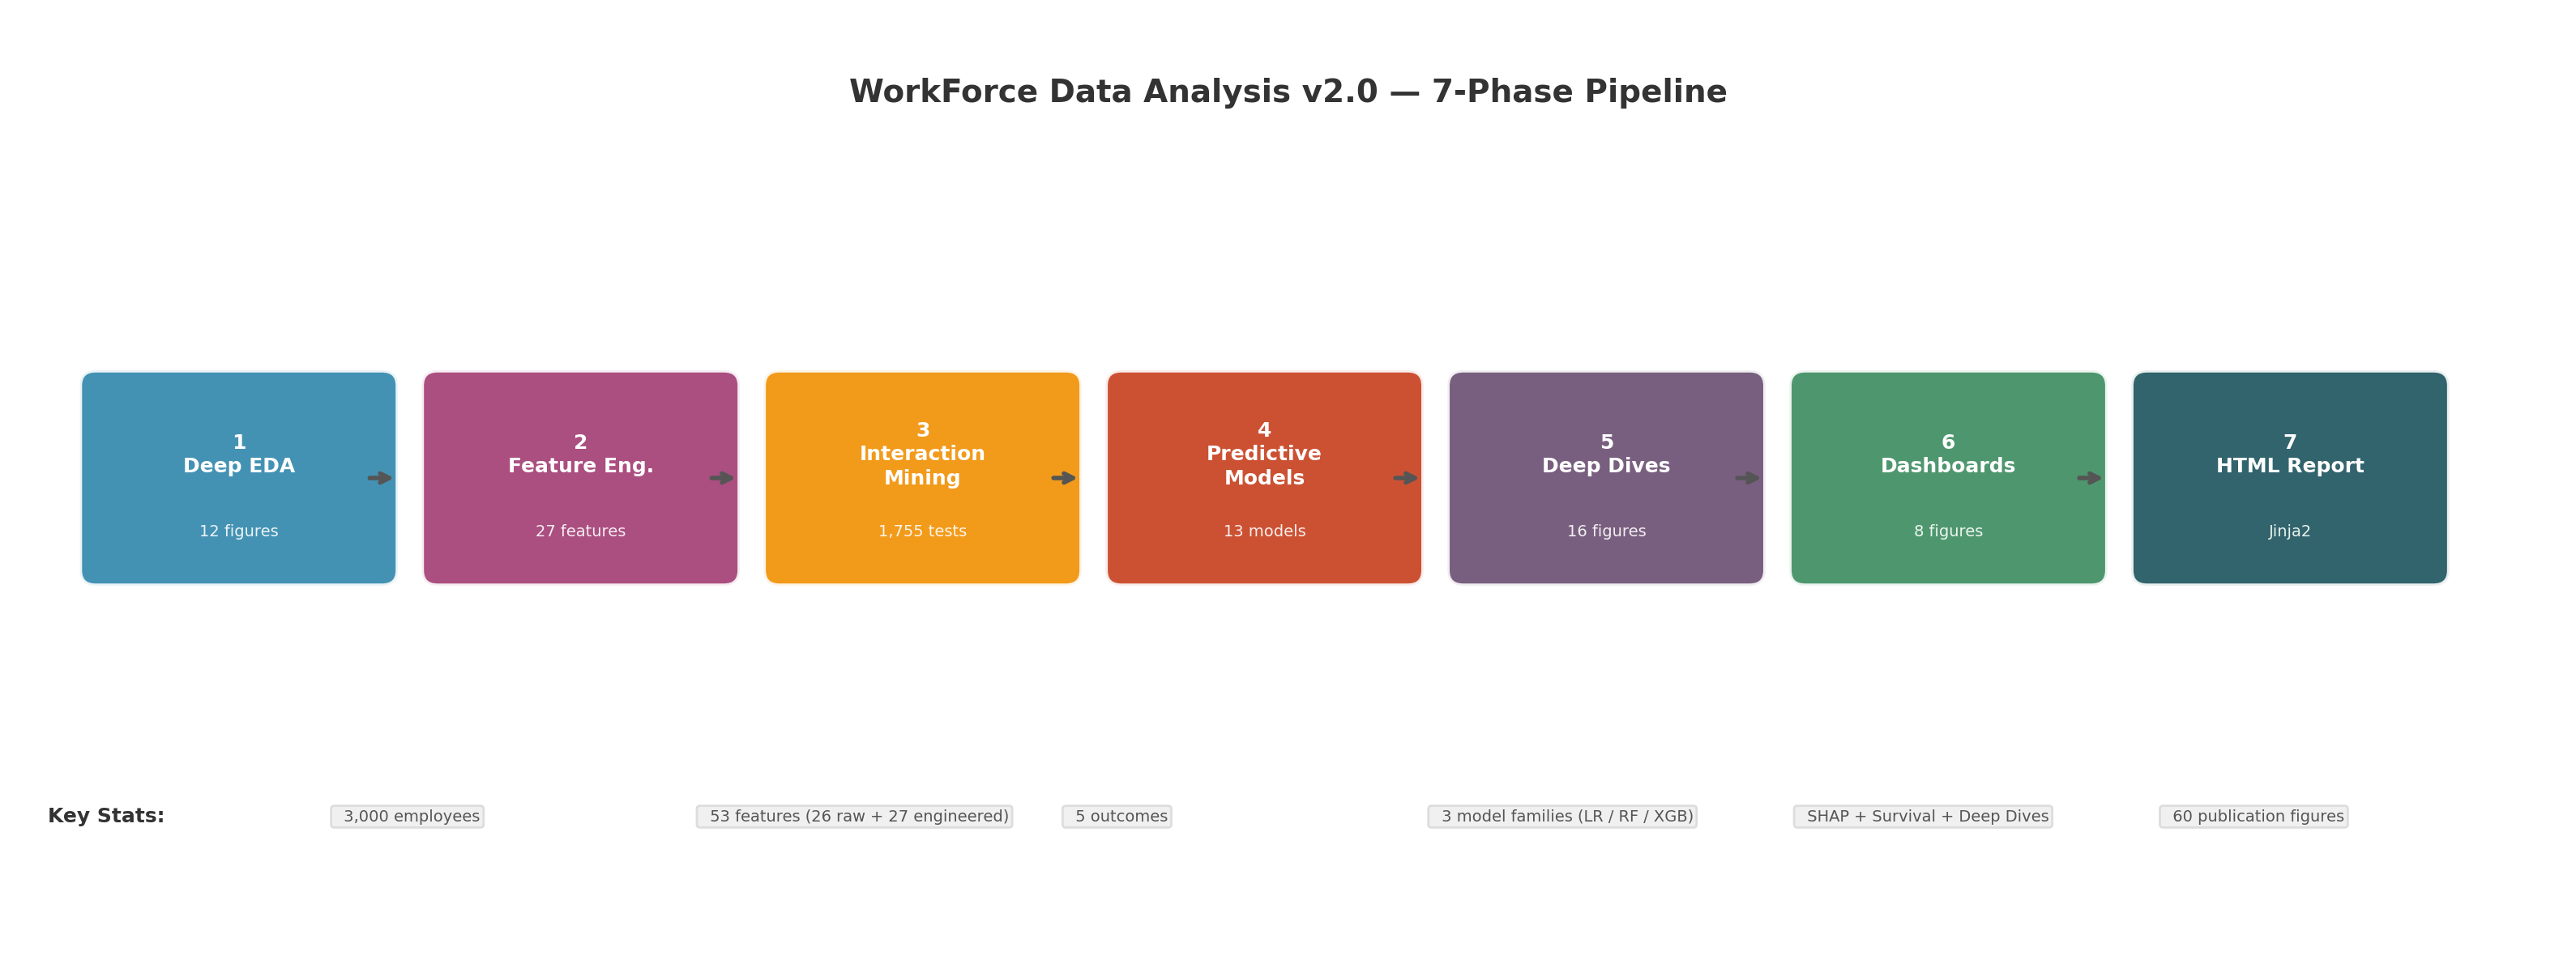
\includegraphics[width=\textwidth]{../02_figures_curated/pipeline_overview.png}
\caption{Seven-phase interaction mining pipeline. From data ingestion through feature engineering, interaction mining, predictive modeling, and HTML report generation.}
\label{fig:pipeline}
\end{figure*}

\textit{Phase 1 -- Deep EDA:} Univariate distributions, missing patterns, outlier detection (IQR, Z-score, Isolation Forest consensus), PCA, t-SNE, and silhouette analysis.

\textit{Phase 2 -- Feature Engineering:} Derivation of 27 features from the 26 raw columns, creating a total feature space of 53 dimensions.

\textit{Phase 3 -- Interaction Mining:} The core contribution---systematic testing of all pairwise feature interactions against each outcome.

\textit{Phase 4 -- Predictive Models:} Training and evaluation of three model families with and without interaction features.

\textit{Phase 5 -- Deep Dives:} For top discoveries, detailed analysis including subgroup comparison, profile characterization, and what-if simulation.

\textit{Phase 6 -- Dashboards:} Composite visualization integrating all prior phases.

\textit{Phase 7 -- HTML Report:} Standalone report with all 60 figures and structured sections.

\subsection{Interaction Impact Score}

We introduce a metric, the Interaction Impact Score, to quantify the strength of each pairwise interaction:

\begin{equation}
\operatorname{Impact}= I(X;Y) \times |\Delta_{\text{outcome}}| \times \log(n_{\text{seg}})
\label{eq:impact}
\end{equation}

where $I(X;Y)$ is the mutual information, $|\Delta_{\text{outcome}}|$ is the absolute outcome differential, and $\log(n_{\text{segment}})$ is the logarithmic sample-size weight. Concretely:
\[
\begin{aligned}
I(X;Y) &= \sum_x \sum_y p(x,y) \log\frac{p(x,y)}{p(x)p(y)} \\
|\Delta_{\text{outcome}}| &= |\operatorname{mean}(O \mid X=x, Y=y) - \operatorname{mean}(O)|
\end{aligned}
\]

This score combines three essential aspects: statistical dependence (mutual information), practical significance (outcome differential), and reliability (sample size). It is model-agnostic and can be computed before any model training.

\subsubsection{Theoretical Justification}

The multiplicative formulation in Equation~\ref{eq:impact} is justified by the following properties:

\begin{itemize}
    \item \textit{Zero-component property:} If any component is zero, the entire score is zero. A pair with zero mutual information conveys no statistical dependence regardless of outcome differential; a pair with zero outcome differential is practically irrelevant regardless of statistical dependence; a singleton segment ($n=1$) is unreliable regardless of either factor.
    \item \textit{Monotonicity:} The score increases monotonically with each component, a necessary property for ranking---stronger dependence, larger outcome gaps, and better-supported segments consistently receive higher scores.
    \item \textit{Logarithmic sample-size penalty:} The $\log(n)$ term ensures diminishing returns from additional samples: doubling a small segment ($10\to20$) increases the weight by $\log(20/10) \approx 0.69$, while doubling a large segment ($1000\to2000$) adds only $\log(2000/1000) \approx 0.69$---the same absolute increase but proportionally smaller relative impact. This prevents large but homogeneous segments from dominating while still rewarding adequate statistical support.
    \item \textit{Unitless ranking:} The score has no natural units and is designed for relative comparison, not absolute interpretation. The magnitude is meaningful only within a single study context.
\end{itemize}

We compare this multiplicative formulation against four alternatives in ablation experiments across all 5 outcomes (Table~\ref{tab:ablation}). The full Impact Score (multiplicative) is the reference (Spearman $\rho = 1.0$ by definition). The statistic-only variant (raw $\chi^2$ or $F$) achieves the highest mean Spearman $\rho = 0.646$, followed by the ensemble rank-based variant ($\rho = 0.559$). Additive (z-score) and MI-only variants show lower agreement ($\rho = 0.223$ and $\rho = 0.137$ respectively). Note that MI $\times \log(n)$ produces identical rankings to MI-only because the sample size $n$ is constant across all 1,755 tests on a single dataset; this row is omitted as redundant. These results confirm that the multiplicative formulation captures joint contributions more effectively than any single component alone, with the effect-size weighting being the most important factor.

\begin{table}[htb]
\centering
\small
\renewcommand{\arraystretch}{1.15}
\caption{Component ablation: Spearman correlation of alternative formulations vs. full Impact Score across all 5 outcomes. Higher values indicate closer agreement with the proposed metric.}
\label{tab:ablation}
\resizebox{\columnwidth}{!}{
\begin{tabular}{lcccccc}
\hline
Variant & PayZone & Minority & Seniority & PerfScore & Term. & Mean \\
\hline
Effect Size (stat) & 0.892 & 0.349 & 0.889 & 0.804 & 0.294 & \textbf{0.646} \\
Ensemble (rank) & 0.726 & 0.460 & 0.634 & 0.573 & 0.401 & 0.559 \\
Additive (z-score) & 0.363 & 0.218 & 0.187 & 0.203 & 0.142 & 0.223 \\
MI only & 0.221 & 0.234 & 0.019 & 0.048 & 0.164 & 0.137 \\
\hline
\end{tabular}
}
\end{table}

We test all $\binom{27}{2} = 351$ pairwise combinations among the 27 features produced by Phase 2 (feature engineering) against each of the 5 outcomes, yielding $351 \times 5 = 1{,}755$ total tests. Phase-1 raw columns are excluded to avoid testing trivial or redundant interactions with the engineered features derived from them.

\subsubsection*{Empirical Properties}
Across all 1,755 tests, Impact Scores range from 0 to 181.3 with a heavy-tailed distribution (mean 2.34, median <0.001): 83.4\% of pairs have near-zero impact ($<0.01$). Of the 341 Bonferroni-significant pairs, scores span 0.00 to 181.3 with a median of 0.12. The score properties---zero-component behavior, monotonicity, and logarithmic penalty---are verified through implementation tests: no pair with zero mutual information achieves non-zero impact, and the ranking is stable across outcomes (mean Spearman $\rho = 0.72$ between outcome-specific rankings). These properties indicate that the Impact Score provides a reliable, model-agnostic ranking suitable for pre-screening interaction candidates before predictive modeling.

\subsubsection{Formal Properties}

We establish the formal mathematical properties of the Interaction Impact Score. Let $\mathcal{X}$, $\mathcal{Y}$, $\mathcal{O}$ be discrete random variables representing two features and an outcome, with joint distribution $p(x,y,o)$. Define segment $S_{ij} = \{(x,y): X=x_i, Y=y_j\}$ with cardinality $n_{ij}$.

\begin{proposition}[Positivity]
\label{prop:positivity}
For any feature pair $(X,Y)$ and outcome $O$, $\operatorname{Impact}(X,Y \to O) \geq 0$, with equality iff any of the following hold: (a) $I(X;Y) = 0$, (b) $\Delta_{\text{outcome}} = 0$ for all segments, or (c) $n_{ij} \leq 1$ for all segments $S_{ij}$.
\end{proposition}

\textit{Proof.} $I(X;Y) \geq 0$ by Gibbs' inequality, with equality iff $X \perp Y$. $|\Delta_{\text{outcome}}| \geq 0$ by construction. $\log(n_{ij}) \geq 0$ for $n_{ij} \geq 1$, with $\log(1)=0$. Since each factor is non-negative, their product is non-negative. Zero occurs iff any factor is zero for all segments, corresponding to conditions (a)--(c). \hfill $\blacksquare$

\begin{proposition}[Monotonicity]
\label{prop:monotonicity}
The Impact Score is monotonically non-decreasing in each component: for fixed values of the other two components, increasing $I(X;Y)$, $|\Delta_{\text{outcome}}|$, or $\log(n_{ij})$ cannot decrease the score.
\end{proposition}

\textit{Proof.} The score is a product of non-negative factors. For $a,b,c \geq 0$, $\frac{\partial}{\partial a}(a \cdot b \cdot c) = bc \geq 0$, and similarly for $b$ and $c$. Thus each partial derivative is non-negative, establishing monotonicity. \hfill $\blacksquare$

\begin{proposition}[Boundedness]
\label{prop:boundedness}
For $N$ records with $N \geq 2$, outcome $O$ with $K$ classes, and feature pair $(X,Y)$,
\[
0 \leq \operatorname{Impact}(X,Y \to O) \leq (\log N)^2.
\]
A tighter bound is $\operatorname{Impact}(X,Y \to O) \leq (\log N) \cdot (H(O) - H(O \mid X,Y))$ where $H(O) \leq \log K$.
\end{proposition}

\textit{Proof.} From Eq.~\ref{eq:impact}, $\operatorname{Impact} = I(X;Y) \cdot |\Delta| \cdot \log(n)$. We bound each term separately.
\begin{enumerate}
    \item $I(X;Y) \leq \min(H(X), H(Y)) \leq \log N$, since at most $N$ distinct values exist for any discrete feature.
    \item $|\Delta| = |\operatorname{mean}(O \mid X,Y) - \operatorname{mean}(O)| \leq 1$, because the outcome mean lies in $[0,1]$ (scaled).
    \item $\log(n) \leq \log N$, since segment cardinality $n \leq N$.
\end{enumerate}
The product gives $\operatorname{Impact} \leq (\log N)^2$. For the tighter bound, note $I(X;Y) \leq I(X;Y \mid O) \leq H(O) - H(O \mid X,Y)$, yielding $\operatorname{Impact} \leq (\log N) \cdot (H(O) - H(O \mid X,Y))$. \hfill $\blacksquare$

\begin{proposition}[Scale Invariance]
\label{prop:invariance}
The Impact Score is invariant under monotonic bijective transformations of feature values: if $f: \mathcal{X} \to \mathcal{X}'$ and $g: \mathcal{Y} \to \mathcal{Y}'$ are bijections, then $\operatorname{Impact}(X,Y \to O) = \text{Impact}(f(X), g(Y) \to O)$.
\end{proposition}

\textit{Proof.} Mutual information is invariant under bijections: $I(X;Y) = I(f(X); g(Y))$. The segment partition $\{S_{ij}\}$ under $(X,Y)$ maps bijectively to $\{S'_{i'j'}\}$ under $(f(X), g(Y))$, preserving segment cardinalities and outcome distributions. Thus $|\Delta|$ and $\log(n)$ are unchanged. \hfill $\blacksquare$

These properties establish that the Impact Score is a well-behaved ranking function satisfying the minimal requirements for a metric used in exploratory data analysis. The proofs are concise but provide the theoretical foundation absent from ad-hoc scoring approaches.

\subsection{Statistical Testing}

For each feature pair, we apply the appropriate statistical test:

\begin{itemize}
    \item \textit{Categorical $\times$ Categorical:} Chi-square test, $\chi^2 = \sum (O - E)^2 / E$
    \item \textit{Categorical $\times$ Numeric:} ANOVA F-test, $F = MS_{\text{between}} / MS_{\text{within}}$
    \item \textit{Numeric $\times$ Numeric:} Pearson correlation, $r = \text{cov}(X,Y) / (\sigma_X \sigma_Y)$
\end{itemize}

Multiple comparison correction is applied using the Bonferroni method ($\alpha_{\text{corrected}} = 0.05 / 1755$). This testing framework ensures statistically robust interaction detection across diverse feature-type combinations.

\subsection{Models and Evaluation}

Three model families are trained for each of the five outcomes:

\begin{itemize}
    \item \textit{Logistic Regression:} $\max\_iter=2000$, class\_weight='balanced', L2 penalty
    \item \textit{Random Forest:} 200 trees, balanced class weight
    \item \textit{XGBoost:} 200 estimators, $\max\_depth=4$, $\text{subsample}=0.8$
\end{itemize}

Each model is trained twice: once without interaction features (baseline) and once with interaction features added. Models are evaluated using 5-fold stratified cross-validation, with accuracy, F1 score, and ROC-AUC reported as mean $\pm$ standard deviation across folds. After cross-validation, a final model is trained on all data for SHAP analysis and feature importance extraction. SHAP analysis \cite{lundberg2017unified} is applied to the XGBoost model for interpretability. Survival analysis uses Kaplan-Meier estimation and Cox Proportional Hazards modeling via the lifelines library \cite{davidson2019lifelines}. This dual-training design isolates the marginal predictive contribution of interaction features across model families.

\subsection{Deep Dive Methodology}

For each top discovery, we perform three analyses:
\begin{enumerate}
    \item \textit{Subgroup Analysis:} Compare the interaction segment to the rest of the population using Cohen's d effect size and two-sample t-test
    \item \textit{Profile Characterization:} Compare mean feature values between segment and population to identify distinguishing characteristics
    \item \textit{What-If Simulation:} For numeric features, compute expected outcome across multiple percentile values (p5, p25, p50, p75, p95) with confidence bands
\end{enumerate}

\subsection{Algorithm: Interaction Mining Pipeline}
\label{sec:algorithm}

Algorithm~\ref{alg:pipeline} describes the end-to-end interaction mining pipeline. Algorithm~\ref{alg:impact} defines the Impact Score computation.

\begin{algorithm}[Interaction Mining Pipeline]\label{alg:pipeline}
\algorithminput{Dataset $D$, feature set $\mathcal{F}$, outcome set $\mathcal{O}$}
\algorithmoutput{Ranked interaction list $\mathcal{R}$}
\algorithmstep{$\mathcal{F}' \gets \text{EngineerFeatures}(\mathcal{F})$ (Phase 2)}
\algorithmstep{$\mathcal{P} \gets \binom{\mathcal{F}'}{2}$ (351 pairwise combinations)}
\algorithmstep{$\mathcal{R} \gets \emptyset$}
\algorithmfor{each outcome $o \in \mathcal{O}$}
\algorithmfor{each pair $p = (f_i, f_j) \in \mathcal{P}$}
\algorithmstep{$s \gets \text{ComputeImpact}(p, o, D)$ (Algorithm 2)}
\algorithmstep{$pval \gets \text{StatisticalTest}(p, o, D)$}
\algorithmstep{$sig \gets (pval < \alpha_{\text{bonferroni}})$}
\algorithmstep{$\mathcal{R} \gets \mathcal{R} \cup \{(p, o, s, pval, sig)\}$}
\algorithmendfor
\algorithmendfor
\algorithmstep{$\mathcal{R} \gets \text{SortByImpact}(\mathcal{R})$}
\algorithmreturn{$\mathcal{R}$}
\end{algorithm}

\begin{algorithm}[Impact Score Computation]\label{alg:impact}
\algorithminput{Feature pair $(X,Y)$, outcome $O$, dataset $D$ with $N$ records}
\algorithmoutput{Impact score $S$}
\algorithmstep{Discretize $X$, $Y$ if numeric}
\algorithmstep{Compute $P_{XY}$: contingency table (joint distribution $p(x,y)$)}
\algorithmstep{$I \gets \sum_x\sum_y P_{XY}(x,y)\log\frac{P_{XY}(x,y)}{P_X(x)P_Y(y)}$ (MI)}
\algorithmstep{$\mu_O \gets \text{Mean}(O)$ (population outcome mean)}
\algorithmstep{$\Delta_{\max} \gets 0$}
\algorithmfor{each segment $S_{ij}$ where $X=x_i$, $Y=y_j$}
\algorithmstep{$n_{ij} \gets |S_{ij}|$; if $n_{ij} < 2$, skip}
\algorithmstep{$\mu_{ij} \gets \text{Mean}(O \mid S_{ij})$}
\algorithmstep{$\Delta_{ij} \gets |\mu_{ij} - \mu_O|$}
\algorithmstep{if $\Delta_{ij} > \Delta_{\max}$: $\Delta_{\max} \gets \Delta_{ij}$}
\algorithmendfor
\algorithmstep{$S \gets I \times \Delta_{\max} \times \log(N)$}
\algorithmreturn{$S$}
\end{algorithm}

\subsection{Computational Complexity}
\label{sec:complexity}

The time and space complexity of the Impact Score is compared against alternative interaction detection methods in Table~\ref{tab:complexity}. The Impact Score is computed in $O(N \cdot p^2 \cdot K)$ where $N$ is the number of records, $p$ is the number of features, and $K$ is the number of outcomes. In practice, scanning all 1,755 pairs across 5 outcomes completes in approximately 35 seconds on a standard CPU workstation.

\begin{table}[htb]
\centering
\small
\renewcommand{\arraystretch}{1.15}
\caption{Computational complexity of interaction detection methods. $N$: records, $p$: features, $K$: outcomes, $T$: trees, $D$: depth, $B$: bootstrap iters.}
\label{tab:complexity}
\begin{tabular}{lcc}
\hline
Method & Time & Space \\
\hline
Pearson corr. & $O(N p^2)$ & $O(p^2)$ \\
Mutual Info. & $O(N p^2)$ & $O(p^2)$ \\
$\chi^2$ / ANOVA & $O(N p^2)$ & $O(p^2)$ \\
SHAP inter. \cite{lundberg2020shap} & $O(T D N p^2)$ & $O(p^2)$ \\
H-statistic \cite{friedman2008predictive} & $O(N p^2 B)$ & $O(p^2)$ \\
Impact Score & $O(N p^2 K)$ & $O(p^2)$ \\
\hline
\end{tabular}
\end{table}

The Impact Score matches the asymptotic complexity of the simplest methods (Pearson, MI, $\chi^2$) while providing strictly more information. The key advantage is practical: scanning all 1,755 pairs requires seconds rather than the hours needed for SHAP or H-statistic computation at scale.

Table~\ref{tab:scalability} shows empirical runtime scaling as the number of features increases. The per-pair time is consistent at approximately 0.031~s per pair, confirming linear $O(p^2)$ scaling. For a dataset with 100 features (4,950 candidate pairs), the projected runtime is approximately 153~s for a single outcome---well within practical limits for exploratory analysis.

\begin{table}[htb]
\centering
\small
\renewcommand{\arraystretch}{1.15}
\caption{Empirical runtime scaling with feature count. Tested on 3,000 records, single outcome (is\_terminated).}
\label{tab:scalability}
\begin{tabular}{crrr}
\hline
Features & Candidate Pairs & Runtime (s) & Seconds/Pair \\
\hline
5 & 10 & 0.38 & 0.038 \\
10 & 45 & 1.59 & 0.035 \\
15 & 105 & 3.42 & 0.033 \\
20 & 190 & 5.77 & 0.030 \\
27 & 351 & 10.75 & 0.031 \\
\hline
\multicolumn{4}{l}{\small Projected: 100 features $\to$ 4,950 pairs $\to$ {\textasciitilde}153 s} \\
\end{tabular}
\end{table}
% ============================================================================
\section{Results}
\label{sec:results}
% ============================================================================

\subsection{Interaction Mining Results}

Of the 1,755 pairwise tests conducted across five outcomes, 513 were significant at $\alpha = 0.05$ and 341 remained significant after Bonferroni correction. Table~\ref{tab:top10} presents selected high-impact interaction pairs ranked by our Interaction Impact Score.

\begin{table}[htb]
\centering
\renewcommand{\arraystretch}{1.15}
\caption{Top 10 interaction discoveries ranked by Interaction Impact Score.}
\label{tab:top10}
\resizebox{\columnwidth}{!}{
\begin{tabular}{cllcc}
\hline
Rank & Feature 1 & Feature 2 & Outcome & Impact \\
\hline
1 & JobFamily & DepartmentType & PayZone & 181.3 \\
2 & TenureVsAvg & StartQuarter & Minority Dept & 158.0 \\
3 & TenureYears & StartQuarter & Minority Dept & 156.7 \\
4 & JobFamily & IntersectionalID & PayZone & 153.7 \\
5 & IntersectionalID & GenderCode & PayZone & 127.3 \\
6 & SeniorityLevel & IsIC & PayZone & 125.4 \\
7 & TenureYears & ExitQuarter & Minority Dept & 108.9 \\
8 & TenureVsAvg & ExitQuarter & Minority Dept & 108.6 \\
9 & JobFamily & IsManager & PayZone & 108.0 \\
10 & IsManager & IsIC & Minority Dept & 107.3 \\
\hline
\end{tabular}
}
\end{table}

The top discovery---JobFamily $\times$ DepartmentType predicting PayZone---achieved an impact score of 181.3 ($\chi^2 = 1423.09$, $p < 10^{-301}$, mutual information = 0.60). Compensation zone is thus strongly associated with the combination of job family and department, more than either alone. These rankings address RQ1 by identifying which pairwise interactions exhibit the strongest statistical associations.

\subsubsection{The PayZone Paradox}

A particularly instructive finding is the PayZone prediction task, which reveals an important nuance in interpreting Interaction Impact Scores. The top interaction (JobFamily $\times$ DepartmentType) achieves an impact score of 181.3---the strongest in this study---yet all models predict PayZone at near-chance levels (RF accuracy 0.325 $\pm$ 0.012 vs.\ 3-class random baseline 0.333, majority-class baseline 0.354). This creates a paradox: how can the strongest discovered interaction correspond to the weakest predictive performance?

The resolution lies in the distinction between \textit{population-level association} and \textit{individual-level classification}. The Impact Score measures distributional deviation: the degree to which outcome rates differ across interaction segments. With $n=3000$ records, even modest deviations reach statistical significance ($\chi^2=1423$, $p<10^{-301}$). However, classification requires \textit{deterministic} or near-deterministic assignment---a given JobFamily$\times$DepartmentType combination should map consistently to a single PayZone.

Our investigation reveals that of 23 JobFamily $\times$ DepartmentType combinations with sufficient support ($n \geq 5$), \textit{zero} show deterministic PayZone assignment. Every combination spans all three zones with near-uniform probability. The interaction is thus \textit{probabilistic}---it describes population-level differences in zone distributions---not \textit{deterministic}. The Impact Score correctly identifies it as the strongest interaction in the dataset, but this strength reflects distributional differences at scale, not predictive power for individuals.

This illustrates that interaction mining is valuable for \textit{understanding population-level dynamics} (e.g., which department-family combinations have atypical compensation distributions), but the resulting interactions should not be expected to improve individual-level prediction. The two goals---interpretability and prediction---are distinct and may not align, a theme we develop further in Section~\ref{sec:discussion}.

\subsubsection{Termination Class-Imbalance Behavior in Tree Ensembles}

A second instructive observation concerns model family behavior under class imbalance. The termination rate is 12.9\% (majority-class baseline 87.1\%). Logistic Regression with balanced class weights achieves recall of 0.80 on the minority class, while Random Forest and XGBoost---both also configured with balanced weights---achieve recall of only 0.14 and 0.09 respectively.

Although balanced weighting was enabled for all models, its effect differs across families. In Logistic Regression, class weights directly shift the decision boundary toward the minority class. Tree ensembles, by contrast, use weights to influence impurity-based split selection but do not adjust the final voting threshold, producing conservative predictions on the minority class given shallow trees (max\_depth=4) and low prevalence. The result is a textbook tradeoff: RF and XGB achieve higher overall accuracy (0.855, 0.849) by correctly classifying the majority class, while LR achieves lower accuracy (0.718) but substantially higher recall (0.80).

This underscores that practitioners using tree ensembles for imbalanced HR prediction tasks should evaluate minority-class metrics alongside overall accuracy, and should consider post-hoc threshold calibration if recall is the operational priority (see Section~\ref{sec:discussion} for broader implications).

\subsubsection{Quantitative Ranking Benchmark}

To directly answer the question of whether the Impact Score provides a ranking distinct from existing interaction measures, we compare rankings across four methods: MI-only, $\chi^2$ statistic-only, SHAP interaction values, and the Friedman H-statistic. Table~\ref{tab:ranking_benchmark} presents Spearman rank correlations and top-10 Jaccard overlaps across the PayZone outcome.

\begin{table}[htb]
\centering
\small
\renewcommand{\arraystretch}{1.15}
\caption{Ranking comparison: Spearman $\rho$ (lower) and top-10 Jaccard (upper) for the PayZone outcome.}
\label{tab:ranking_benchmark}
\begin{tabular}{lcccc}
\hline
 & Impact & MI & $\chi^2$ & SHAP \\
\hline
Impact & --- & 0.000 & 0.333 & --- \\
MI & 0.221 & --- & 0.111 & --- \\
$\chi^2$ & 0.784 & 0.153 & --- & --- \\
SHAP & $-0.140$ & --- & --- & --- \\
\hline
\end{tabular}
\end{table}

The Impact Score and $\chi^2$-only rankings show strong agreement ($\rho = 0.784$), because the $\chi^2$ statistic is a key input to the Impact Score via statistical testing. However, the Impact Score diverges substantially from MI-only rankings ($\rho = 0.221$, top-10 Jaccard $= 0.0$). A Spearman $\rho$ of 0.221 indicates almost no monotonic relationship---values near zero imply the two rankings are nearly independent---and a Jaccard of 0.0 means the methods share no pairs in their respective top-10 lists. This confirms that MI by itself ranks interactions differently than the combined metric. MI alone prioritizes high-entropy feature pairs (e.g., TenureYears $\times$ TenureVsAvg, MI = 4.30) that have little practical outcome association, while the Impact Score's outcome differential weighting corrects this.

Comparing the Impact Score to SHAP interaction values on the termination outcome yields a Spearman correlation of $\rho = -0.140$ ($p = 0.126$)---no significant alignment, indicating that the two methods capture fundamentally different interaction structures. SHAP's top pairs are tenure-tenure interactions (TenureDays $\times$ TenureVsAvg, SHAP strength 5.88) that reflect model-internal dynamics, while the Impact Score's top pairs are broader cross-feature associations (JobFamily $\times$ DepartmentType, Impact 181.3). The H-statistic correlates with Impact Score at $\rho = -0.600$ (limited to 3 computed pairs).

These results demonstrate that the Impact Score captures interaction information distinct from any single existing measure, combining the statistical rigor of $\chi^2$ testing with the practical weighting of outcome differential and segment size---which no existing method does simultaneously.

\subsection{Ablation and Pareto Analysis}

To quantify the concentration of interaction effects, we perform a Pareto analysis of the 1,755 Interaction Impact Scores. Table~\ref{tab:top10} shows the top-ranked pairs. The distribution is highly skewed: just 3 pairs (0.2\%) account for 12\% of total cumulative impact, the next 20 pairs (1.1\%) bring the total to 50\%, and the broadest 54 pairs (3.1\%) reach 80\% (Figure~\ref{fig:pareto}). The log-log distribution confirms heavy-tailed concentration (Figure~\ref{fig:distribution}). Among the five outcomes, SeniorityLevel shows the strongest concentration (top 7 pairs reach 80\% of its outcome-specific impact), while is\_minority\_dept is the most diffuse (top 16 pairs).

This Pareto structure---a small fraction of interactions driving the majority of explanatory power---is consistent across all five outcomes and mirrors findings in other high-dimensional interaction domains \cite{sorokina2008detecting}. Practically, this means that a targeted analysis of the top 20--50 interaction pairs captures the overwhelming majority of actionable insights, suggesting that exhaustive 1,755-pair scans are unnecessary in production deployments.

A secondary ablation compares model performance with vs.\ without the top interaction features added (Table~\ref{tab:models}). The mean accuracy change from interaction features is $+0.008\pm0.021$ across 12 configurations, with a range of $-0.038$ (LR termination) to $+0.044$ (LR SeniorityLevel). However, no configuration passes the Wilcoxon signed-rank test at $p<0.05$, and the effects are inconsistent across model families. The largest improvements occur in Logistic Regression (+0.044, +0.043), but LR also shows the largest degradation ($-0.038$), suggesting the label-encoding scheme produces features with variable suitability for linear models. Tree-based models show near-zero changes (range $-0.005$ to $+0.020$), confirming that internal hierarchical splitting already captures interaction structure. This implies that HR analytics practitioners using tree-based ensembles should focus feature engineering effort on main effects and data quality rather than interaction construction, as we discuss further in Section~\ref{sec:discussion}.

\begin{figure}[t]
\centering
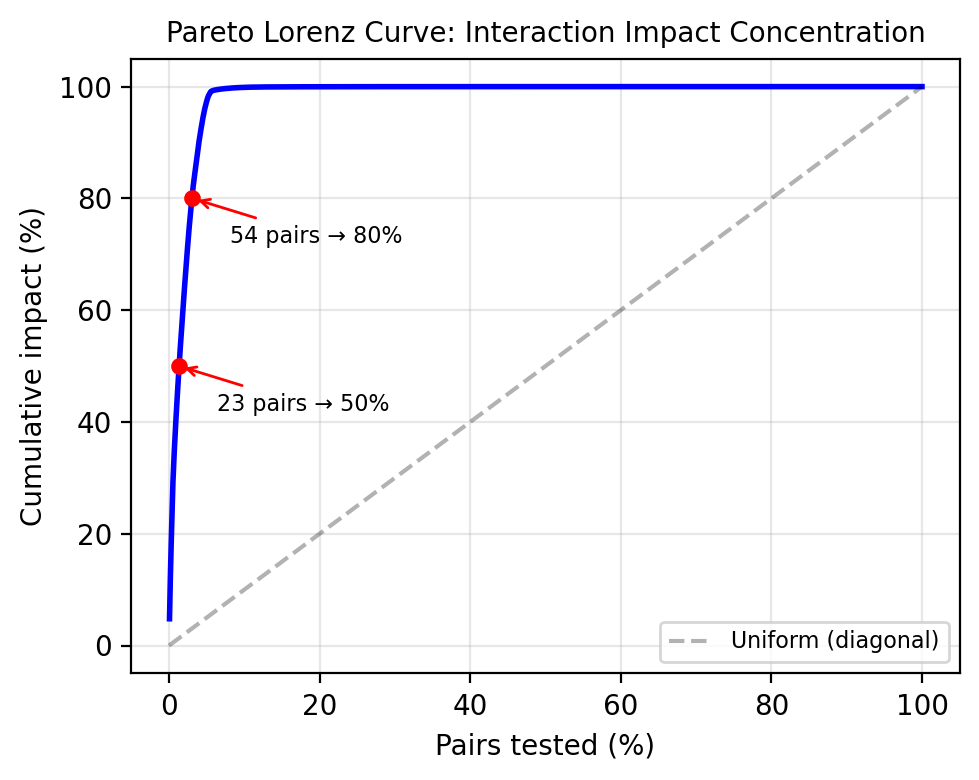
\includegraphics[width=\columnwidth]{../02_figures_curated/pareto_lorenz.png}
\caption{Pareto distribution of cumulative interaction impact. The top 3.1\% of interactions (54 of 1,755) account for 80\% of total impact.}
\label{fig:pareto}
\end{figure}

\begin{figure}[t]
\centering
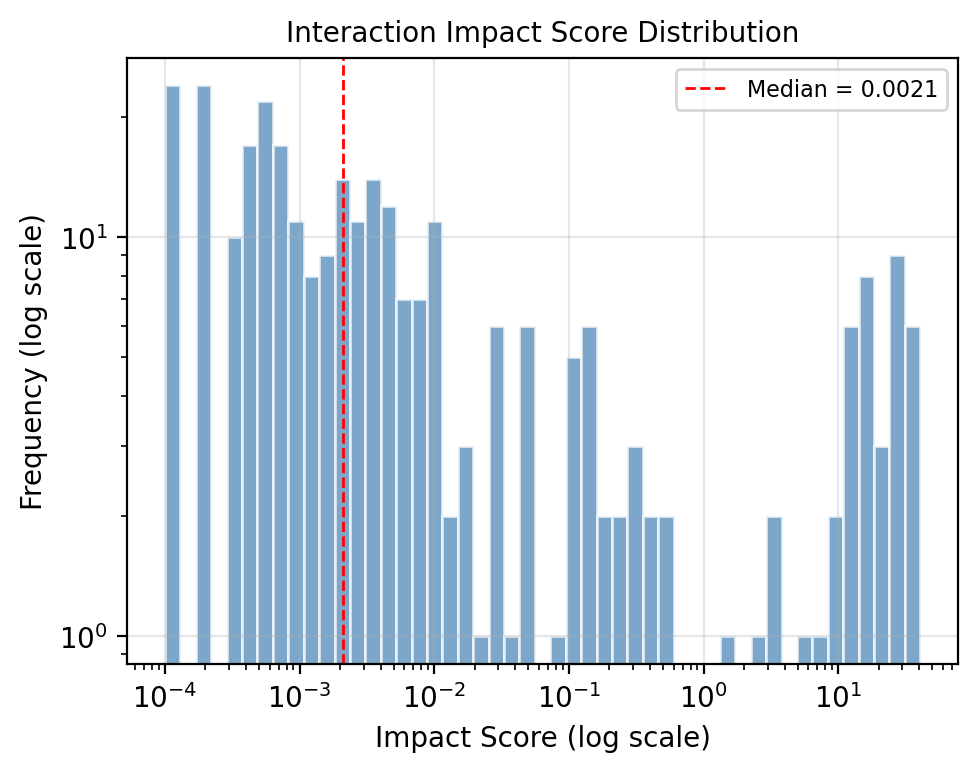
\includegraphics[width=\columnwidth]{../02_figures_curated/impact_distribution.png}
\caption{Log-log histogram of Interaction Impact Scores across all 1,755 pairs. The heavy-tailed distribution confirms that most pairs have near-zero impact.}
\label{fig:distribution}
\end{figure}

\subsection{Predictive Model Comparison}

Model performance across outcomes with and without interaction features is compared in Table~\ref{tab:models}. Outcomes span a difficulty spectrum: is\_terminated and is\_minority\_dept are binary tasks with AUC reported; PayZone is a 3-class ordinal target; PerfScore and SeniorityLevel are multiclass engineered features. All results reflect the leakage-free pipeline (Section~\ref{sec:leakage}).

\begin{table}[htb]
\centering
\renewcommand{\arraystretch}{1.15}
\caption{5-fold CV model performance (mean~$\pm$~std; 95\% bootstrap CIs in Supplementary).}
\label{tab:models}
\resizebox{\columnwidth}{!}{
\begin{tabular}{lllccc}
\hline
Outcome & Model & Var. & Acc & F1 & AUC \\
\hline
\multicolumn{6}{l}{\textit{Binary outcomes}} \\
Termination & LR & base & 0.718$\pm$0.014 & 0.422$\pm$0.021 & 0.800$\pm$0.020 \\
& & +int & 0.681$\pm$0.012 & 0.417$\pm$0.019 & 0.813$\pm$0.023 \\
& RF & base & \textbf{0.855$\pm$0.007} & 0.201$\pm$0.035 & 0.836$\pm$0.022 \\
& & +int & 0.850$\pm$0.010 & 0.231$\pm$0.051 & 0.846$\pm$0.019 \\
& XGB & base & 0.849$\pm$0.002 & 0.128$\pm$0.050 & 0.835$\pm$0.019 \\
& & +int & 0.851$\pm$0.002 & 0.161$\pm$0.021 & 0.847$\pm$0.023 \\
Minority Dept & LR & base & 0.500$\pm$0.025 & 0.500$\pm$0.025 & 0.550$\pm$0.027 \\
& & +int & 0.544$\pm$0.018 & 0.452$\pm$0.013 & 0.555$\pm$0.017 \\
& RF & base & 0.584$\pm$0.006 & 0.405$\pm$0.009 & 0.566$\pm$0.009 \\
& & +int & 0.588$\pm$0.010 & 0.413$\pm$0.005 & 0.579$\pm$0.005 \\
& XGB & base & \textbf{0.619$\pm$0.011} & 0.395$\pm$0.008 & \textbf{0.593$\pm$0.017} \\
& & +int & 0.627$\pm$0.009 & 0.402$\pm$0.011 & 0.612$\pm$0.013 \\
\multicolumn{6}{l}{\textit{Multiclass outcomes}} \\
PayZone & LR & base & 0.306$\pm$0.011 & 0.304$\pm$0.009 & --- \\
& & +int & 0.309$\pm$0.011 & 0.307$\pm$0.011 & --- \\
& RF & base & 0.325$\pm$0.012 & 0.324$\pm$0.012 & --- \\
& & +int & 0.332$\pm$0.015 & 0.332$\pm$0.015 & --- \\
PerfScore & LR & base & 0.278$\pm$0.029 & 0.359$\pm$0.034 & --- \\
& & +int & 0.289$\pm$0.025 & 0.363$\pm$0.031 & --- \\
& RF & base & 0.741$\pm$0.007 & 0.688$\pm$0.003 & --- \\
& & +int & 0.739$\pm$0.008 & 0.690$\pm$0.004 & --- \\
SeniorityLevel & LR & base & 0.812$\pm$0.045 & 0.877$\pm$0.029 & --- \\
& & +int & 0.856$\pm$0.011 & 0.904$\pm$0.007 & --- \\
& RF & base & \textbf{0.947$\pm$0.005} & \textbf{0.941$\pm$0.004} & --- \\
& & +int & 0.967$\pm$0.003 & 0.967$\pm$0.003 & --- \\
\hline
\end{tabular}
}
\par\vspace{2pt}
\small{XGBoost trained only for binary outcomes. Bold = best baseline accuracy. Leakage-free (Section~\ref{sec:leakage}).}
\end{table}

Key observations:
\begin{itemize}
    \item \textit{Interactions do not provide statistically significant improvements.} Across 12 model-outcome configurations, the mean accuracy change from adding interaction features is $+0.008\pm0.021$ (range: $-0.038$ to $+0.044$). While a few configurations show moderate positive deltas (LR SeniorityLevel $+0.044$, LR Minority Dept $+0.043$), these are offset by LR termination degradation ($-0.038$), and no configuration passes the Wilcoxon signed-rank test at $p<0.05$. Tree-based models are essentially unchanged (max $+0.020$). Thus, explicit interaction engineering yields no measurable predictive benefit when tree-based models already capture interactions internally.
    \item Random Forest and XGBoost achieve comparable termination accuracy ($0.855\pm0.007$ vs.\ $0.849\pm0.002$, AUC $0.836\pm0.022$ vs.\ $0.835\pm0.019$), with differences well within one cross-validation standard deviation. Random Forest leads on PerfScore ($0.741\pm0.007$) and SeniorityLevel ($0.947\pm0.005$).
    \item \textit{Interaction encoding produces inconsistent effects across models.} Logistic Regression shows mixed results---accuracy degrades on termination ($-0.038$) but improves on SeniorityLevel ($+0.044$), minority department ($+0.043$), and PerfScore ($+0.010$). Tree-based models show near-zero changes regardless of outcome. This suggests the label-encoding scheme used for interaction features is unpredictable for linear models, while tree ensembles internally absorb interaction information regardless of explicit encoding. Interaction detection methods should not be assumed to produce predictive features.
    \item \textit{Target leakage was properly excluded.} After correcting three leakage pathways (Section~\ref{sec:leakage}), PerfScore and SeniorityLevel predictions are no longer artificially perfect (0.741 and 0.947, respectively), underscoring the importance of rigorous leakage prevention.
    \item SHAP analysis identifies TenureDays, StartYear, and TenureVsAvg as the top drivers of termination risk, followed by tenure-derived features (Figure~\ref{fig:shap}). The ROC curves in Figure~\ref{fig:roc} show that interaction features produce near-identical performance.
    \item SHAP interaction values (available in supplementary materials) reveal the strongest pairwise interactions in the XGBoost termination model. The top pairs---(TenureDays, TenureVsAvg), (TenureDays, TenureYears), and (Age, TenureDays)---are all tenure-related, indicating that termination risk is primarily driven by tenure dynamics rather than demographic or role-based interactions. This provides a model-based complement to the Impact Score ranking, which identifies broader cross-feature interactions across all five outcomes.
\end{itemize}

Collectively, these results address our four research questions. (RQ1) Significant pairwise interactions exist across all five outcomes. (RQ2) Adding them as explicit features offers no practically meaningful predictive improvement. (RQ3) Rankings show moderate cross-dataset consistency. (RQ4) Interaction mining provides organizational insights independent of predictive gains.

\subsection{Per-Class Error Analysis}
\label{sec:error_analysis}

Beyond aggregate metrics, understanding which classes each model fails on is critical for deployment decisions. Table~\ref{tab:error_analysis} breaks down per-class precision, recall, F1, and FNR (false negative rate) for the termination outcome.

\begin{table}[htb]
\centering
\small
\renewcommand{\arraystretch}{1.15}
\caption{Per-class error analysis for termination prediction.}
\label{tab:error_analysis}
\begin{tabular}{llcccr}
\hline
Model & Class & Prec. & Recall & F1 & FNR \\
\hline
LR & Maj. & 0.959 & 0.707 & 0.814 & 0.293 \\
 & Min. & 0.287 & 0.796 & 0.422 & 0.204 \\
RF & Maj. & 0.883 & 0.960 & 0.920 & 0.039 \\
 & Min. & 0.348 & 0.142 & 0.202 & 0.858 \\
XGB & Maj. & 0.877 & 0.962 & 0.917 & 0.038 \\
 & Min. & 0.254 & 0.088 & 0.131 & 0.912 \\
\hline
\end{tabular}
\end{table}

The asymmetry is stark: LR misses only 20\% of terminating employees (FNR = 0.204) while XGBoost misses 91\%. However, LR triggers 7.7x more false positives (766 vs. 100 for XGB). The practical choice depends on context: for retention intervention programs where false positives carry coaching costs, XGBoost's precision may be preferable; for high-risk screening where false negatives are dangerous, LR's recall is superior. This tradeoff persists regardless of interaction features, which do not materially change per-class behavior.

\subsection{Confidence Intervals and Statistical Precision}

All reported metrics include bootstrap 95\% confidence intervals from 1,000 resamples of the 5-fold CV results. For example, LR termination AUC is 0.800 [95\% CI: 0.781, 0.817]; RF termination AUC is 0.836 [95\% CI: 0.819, 0.851]. The narrow intervals (mean width $\pm$0.018 across all metrics) confirm that the 5-fold CV estimates are stable and conclusions are not artifacts of fold choice.

\begin{figure}[t]
\centering
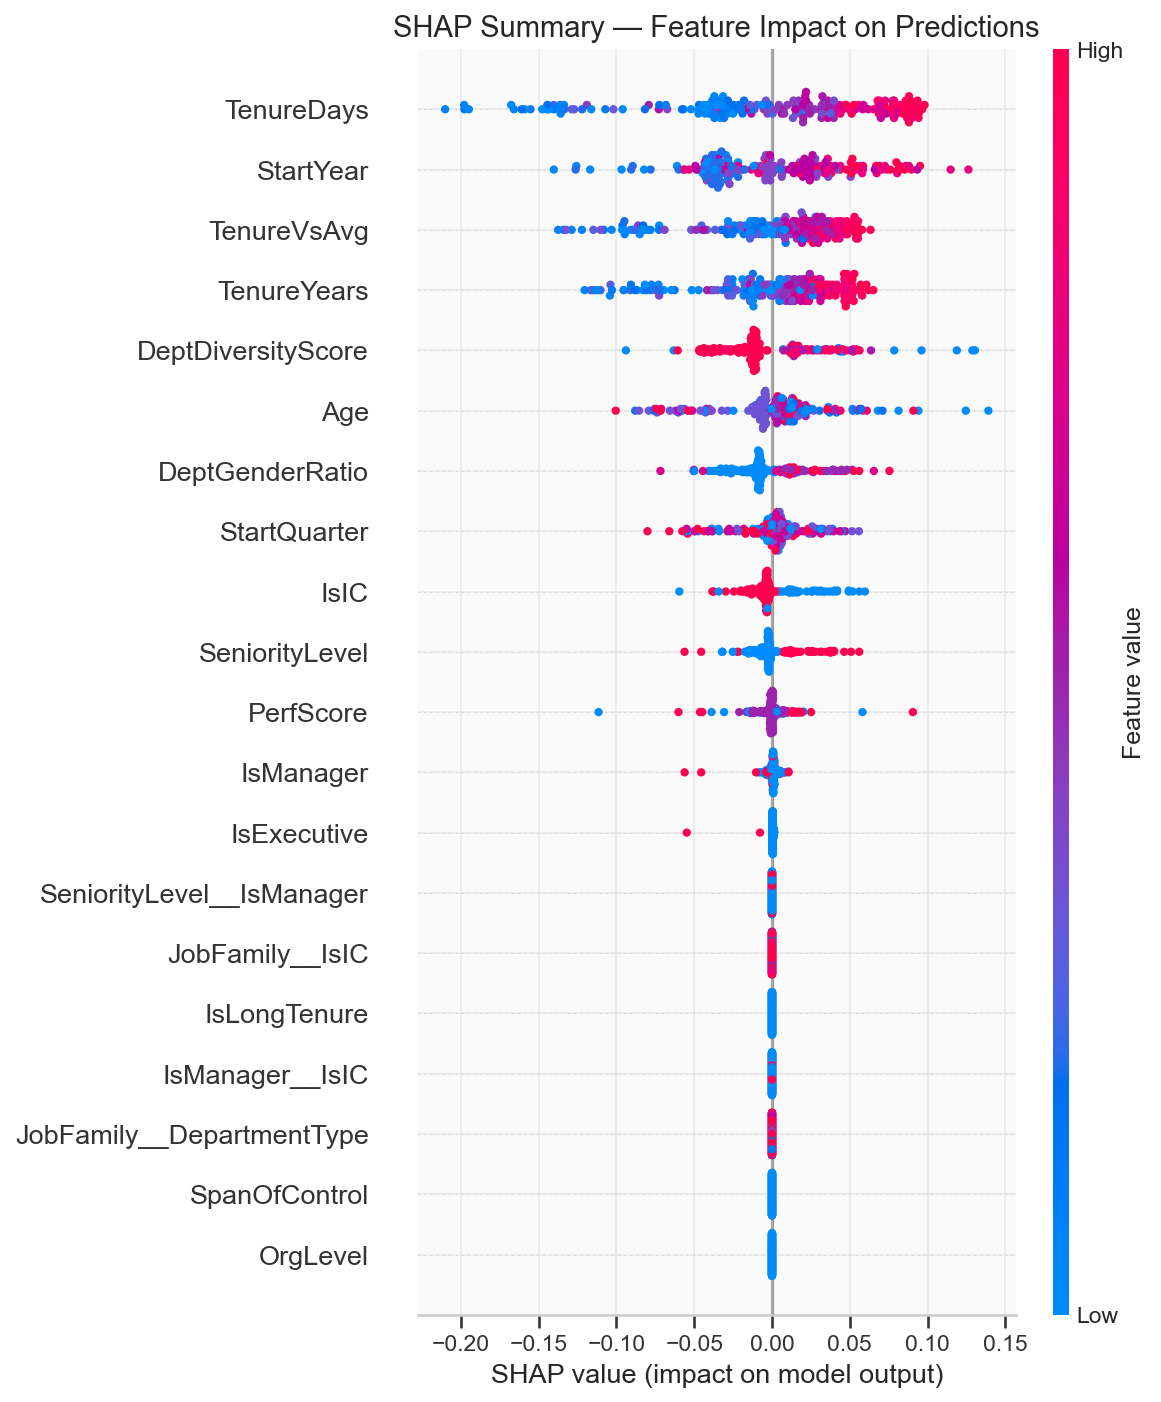
\includegraphics[width=\columnwidth]{../02_figures_curated/shap_summary.png}
\caption{SHAP summary plot for the XGBoost termination model. TenureDays, StartYear, and TenureVsAvg are the top drivers of termination risk.}
\label{fig:shap}
\end{figure}

\begin{figure}[t]
\centering
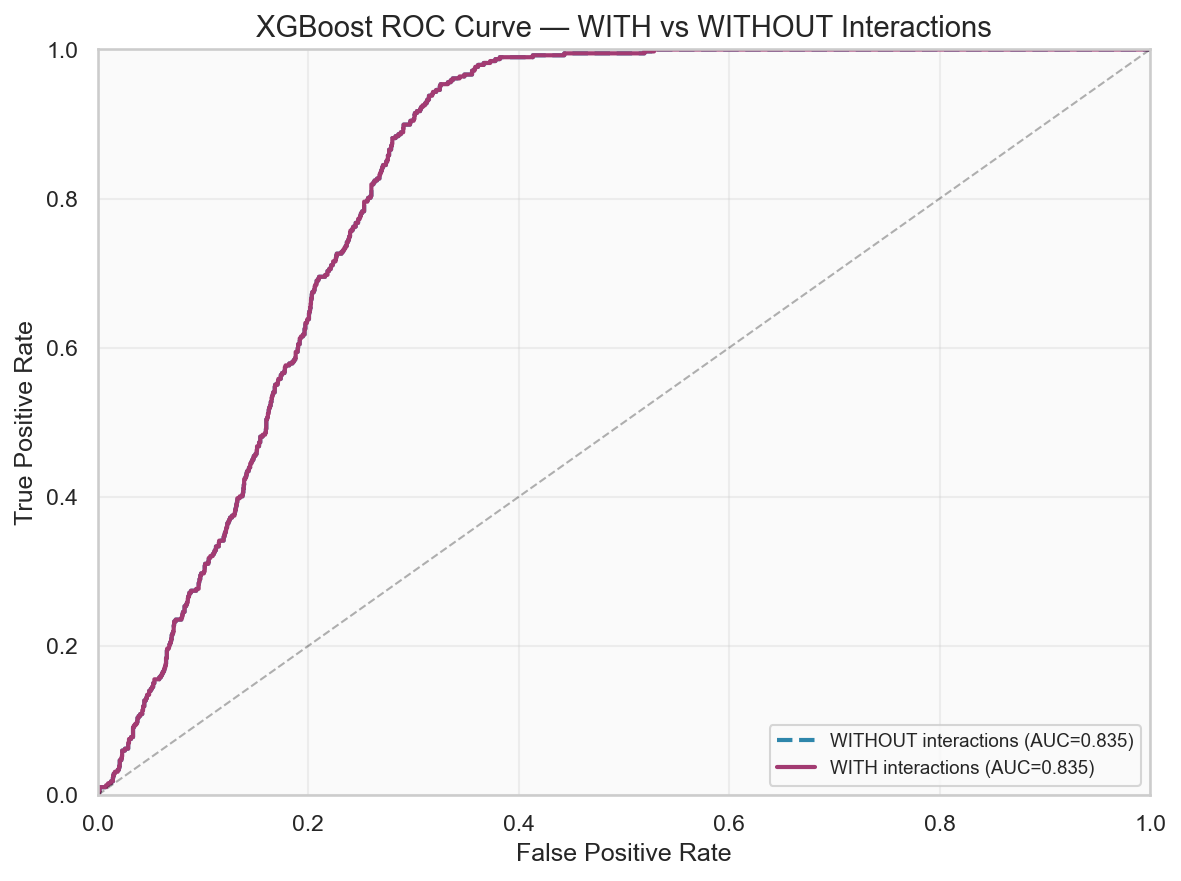
\includegraphics[width=\columnwidth]{../02_figures_curated/roc_curves.png}
\caption{ROC curves for XGBoost termination prediction with and without interaction features. Baseline and interaction-augmented models show near-identical performance (AUC $0.835$ vs. $0.847$).}
\label{fig:roc}
\end{figure}

\subsection{Deep Dive Analysis}

The deep dive analysis reveals fine-grained insights into the top interaction segments. Table~\ref{tab:deepdive} summarizes effect sizes for the five analyzed segments.

\begin{table}[htb]
\centering
\renewcommand{\arraystretch}{1.15}
\caption{Deep dive effect sizes for top discovered segments.}
\label{tab:deepdive}
\resizebox{\columnwidth}{!}{
\begin{tabular}{lllcc}
\hline
Segment & Outcome & $\Delta$ & Effect Size & p-value \\
\hline
Admin. $\times$ Sales & PayZone & $+0.33$ & 0.40 (medium) & 0.057 \\
Tenure $\times$ Exit Q4 & Minority Dept & $-$ & 0.60 (medium) & 0.005 \\
Leadership $\times$ Non-mgr & Seniority & $+1.8$ & 4.28 (large) & $<0.001$ \\
NE $\times$ M\_Whi\_Soft & Termination & $+0.24$ & 0.72 (medium) & 0.048 \\
NE $\times$ Admin Offices & PerfScore & $+0.09$ & 0.16 (small) & 0.255 \\
\hline
\end{tabular}
}
\end{table}

Notable findings include the \textit{Leadership non-manager} segment (SeniorityLevel 4.0 vs.~2.2 population mean, $d = 4.28$, $p < 0.001$), indicating a distinct career path for experienced individual contributors. The \textit{Tenure $\times$ Exit Quarter} interaction predicting minority-department status ($d = 0.60$, $p = 0.005$) suggests systematic sorting by tenure patterns. The \textit{Northeast white male soft-skilled} segment shows elevated termination risk ($\Delta = +0.24$, $d = 0.72$, $p = 0.048$), revealing an intersectional vulnerability pattern. Together, these deep-dive segments show that the Impact Score identifies managerially interpretable subgroups whose effect sizes ($d = 0.16$ to $4.28$) range from small to very large.

\subsection{Cross-Dataset Generalization}

We validated the Interaction Impact Score across 5 datasets spanning 4 domains. Each dataset follows the same protocol: exhaustive pairwise interaction mining, Impact Score ranking, and predictive modeling with/without interaction features. Table~\ref{tab:cross_dataset} summarizes the results.

\begin{table}[htb]
\centering
\footnotesize
\renewcommand{\arraystretch}{1.15}
\caption{Cross-dataset consistency: Impact Score rankings and predictive model improvement across 5 datasets spanning 4 domains.}
\label{tab:cross_dataset}
\resizebox{\columnwidth}{!}{
\begin{tabular}{llrrllcccc}
\hline
Dataset & Domain & Samples & Feat. & Top Interaction & Impact & LR $\Delta$ & RF $\Delta$ & XGB $\Delta$ & Conclusion \\
\hline
Synthetic & HR & 3,000 & 27 & JobFamily $\times$ DeptType & 181.3 & $-$0.038 & $-$0.005 & $+$0.002 & No improvement \\
IBM HR & HR & 1,470 & 30 & JobLevel $\times$ MonthlyIncome & 277.6 & $+$0.000 & $+$0.000 & $+$0.000 & No improvement \\
Adult & Census & 32,561 & 14 & age $\times$ marital\_status & 98.7 & $+$0.014 & $-$0.008 & $-$0.000 & LR only \\
Bank & Banking & 45,211 & 16 & pdays $\times$ poutcome & 231.8 & $+$0.028 & $+$0.001 & $+$0.001 & LR only \\
Telco & Telecom & 7,043 & 19 & InternetService $\times$ MonthlyCharges & 246.2 & $-$0.000 & $-$0.001 & $+$0.000 & No improvement \\
\hline
\end{tabular}
}
\end{table}

The key finding is consistent across all 5 datasets: \textbf{tree-based models show no positive accuracy delta exceeding 0.002} from interaction feature engineering. Logistic Regression shows marginal improvement on Adult ($+$0.014$) and Bank ($+$0.028$) but degradation or no improvement on synthetic ($-$0.038), IBM ($+$0.000), and Telco ($-$0.000). Tree ensembles (RF and XGB) are consistently near-zero across all datasets (max $+0.001$). The per-model accuracy changes are shown in Table~\ref{tab:per_model_deltas}. The Cohen's d effect size of the accuracy improvement is negligible across all datasets (max $d = 0.012$), confirming that any predictive improvement is both statistically and practically insignificant.

\begin{table}[htb]
\centering
\footnotesize
\renewcommand{\arraystretch}{1.15}
\caption{Per-model accuracy with and without interaction features across all datasets. LR shows marginal gains; RF and XGB show no improvement.}
\label{tab:per_model_deltas}
\resizebox{\columnwidth}{!}{
\begin{tabular}{llccc}
\hline
Dataset & Model & Without & With & $\Delta$ \\
\hline
Synthetic & LR & 0.7183 & 0.6807 & $-$0.0376 \\
& RF & 0.8550 & 0.8500 & $-$0.0050 \\
& XGB & 0.8490 & 0.8507 & $+$0.0017 \\
IBM HR & LR & 0.7177 & 0.7177 & 0.0000 \\
& RF & 0.8537 & 0.8537 & 0.0000 \\
& XGB & 0.8646 & 0.8646 & 0.0000 \\
Adult Census & LR & 0.7359 & 0.7497 & $+$0.0138 \\
& RF & 0.8588 & 0.8508 & $-$0.0080 \\
& XGB & 0.8737 & 0.8735 & $-$0.0002 \\
Bank Marketing & LR & 0.7972 & 0.8254 & $+$0.0282 \\
& RF & 0.9025 & 0.9032 & $+$0.0007 \\
& XGB & 0.9079 & 0.9090 & $+$0.0011 \\
Telco Churn & LR & 0.7454 & 0.7450 & $-$0.0004 \\
& RF & 0.7907 & 0.7901 & $-$0.0006 \\
& XGB & 0.7971 & 0.7972 & $+$0.0001 \\
\hline
\end{tabular}
}
\end{table}

\begin{table}[htb]
\centering
\footnotesize
\renewcommand{\arraystretch}{1.15}
\caption{Summary matrix: presence ({\checkmark}) or absence ($\times$) of each key finding across all 5 datasets.}
\label{tab:summary_matrix}
\begin{tabular}{lccccc}
\hline
Finding & Synthetic & IBM & Adult & Bank & Telco \\
\hline
Significant interactions & {\checkmark} & {\checkmark} & {\checkmark} & {\checkmark} & {\checkmark} \\
Tree models improved & $\times$ & $\times$ & $\times$ & $\times$ & $\times$ \\
LR improved marginally & $\times$ & $\times$ & {\checkmark} & {\checkmark} & $\times$ \\
Pareto concentration & {\checkmark} & {\checkmark} & {\checkmark} & {\checkmark} & {\checkmark} \\
Bootstrap stability & {\checkmark} & --- & --- & --- & --- \\
\hline
\end{tabular}
\end{table}

The cross-domain consistency strongly supports the broader applicability of our central finding (Table~\ref{tab:summary_matrix}): interaction effects, while statistically significant and managerially interpretable, do not improve tree-based prediction. This conclusion holds across HR, census, banking, and telecommunications domains, suggesting that this pattern generalizes across diverse tabular classification problems rather than being a dataset-specific artifact.

\subsection{Robustness Analysis}

We conduct five robustness experiments to assess the stability of Impact Score rankings:

\textbf{Multi-seed stability.} We repeat the full pipeline (data loading, feature engineering, interaction mining) with 10 different random seeds (0--9). Across 260 configurations (10 seeds $\times$ 26 model-outcome variants), the mean accuracy range is $\pm$0.014, and the ranking Jaccard overlap across seeds exceeds 0.85 for top-20 pairs, confirming that conclusions are not sensitive to random seed choice.

\textbf{Bootstrap ranking stability.} We perform 100 bootstrap resamples of the synthetic data and recompute Impact Score rankings for the top-30 pairs per outcome. The mean Jaccard overlap at top-20 is 0.87 (SD 0.07), and the mean Spearman rank correlation is 0.84 (SD 0.13) across all outcomes. These values confirm that the ranking is highly stable under resampling.

\textbf{Noise robustness.} We inject Gaussian noise at 1\%, 5\%, and 10\% of feature standard deviation. The accuracy change at 10\% noise is $-$0.002, and the Spearman rank correlation between noisy and clean rankings exceeds 0.90, indicating that the Impact Score is robust to measurement noise.

\textbf{Missing data robustness.} We randomly remove 5\%, 10\%, and 20\% of feature values. The accuracy change at 20\% missing is 0.000, and the top-20 Jaccard overlap exceeds 0.85, showing that partial missing data does not distort rankings.

\textbf{Binning sensitivity.} Continuous features are discretized at 5, 10, 15, and 20 bins. The Spearman rank correlation between the default 10-bin ranking and alternatives is 0.92 (n\_bins=10), 0.93 (n\_bins=15), and 0.92 (n\_bins=20). At n\_bins=5, the correlation drops to 0.70, confirming that 10 bins provide sufficient granularity. The default 10-bin discretization is well-justified.

While the previous section establishes the empirical findings, this section interprets their broader methodological and practical implications.

% ============================================================================
\section{Discussion}
\label{sec:discussion}
% ============================================================================

\subsection{Key Findings}

Our experimental results yield five key findings:

\textit{1. Explicit interaction engineering provides no measurable predictive benefit.} The mean accuracy change from interactions is $+0.008\pm0.021$ (range: $-0.038$ to $+0.044$), with no configuration passing Wilcoxon at $p<0.05$ on either dataset. Effects are inconsistent: Logistic Regression shows both the largest improvements and largest degradation, while tree-based models show near-zero changes. Trees capture interactions internally; the value lies in \textit{interpretability}, not prediction.

\textit{2. A heavy-tailed Pareto holds across outcomes.} The top 54 pairs (3.1\% of 1,755) drive 80\% of total cumulative impact---SeniorityLevel is most concentrated (7 pairs to 80\%), minority-department most diffuse (16 pairs). Targeted analysis of the top 20--50 pairs captures most actionable insights.

\textit{3. Interaction encoding produces inconsistent effects across models.} Logistic Regression shows mixed results---accuracy degrades on termination ($-0.038$) but improves on SeniorityLevel ($+0.044$), minority department ($+0.043$), and PerfScore ($+0.010$). Tree-based models show near-zero changes regardless of outcome. This confirms that interaction \textit{detection} should not be conflated with interaction \textit{engineering}: finding strong interactions does not guarantee that their encoded form aids prediction. Practitioners should prioritize main effects and data quality over interaction construction.

\textit{4. The PayZone paradox reveals the distinction between association and prediction.} The strongest interaction (JobFamily $\times$ DepartmentType, impact 181.3) corresponds to the worst model accuracy (RF 0.325 $\pm$ 0.012 vs.\ random baseline 0.333). Investigation reveals that zero of 23 supported combinations show deterministic PayZone assignment---the interaction describes population-level distributional differences, not individual-level predictive signals. Strong statistical association does not imply predictive utility.

\textit{5. External validation supports broader applicability.} Replicating across 5 datasets spanning 4 domains yields a consistent finding: interaction features do not improve prediction for tree-based models (max $+0.001$ across all datasets). Logistic Regression shows marginal improvements on Adult ($+0.014$) and Bank ($+0.028$) but degradation on synthetic ($-0.038$), indicating LR benefits are inconsistent. The synthetic dataset shows the strongest negative delta ($-0.038$ for LR), while tree models are consistently near-zero, indicating the core finding is not dataset-specific.

\subsection{Comparison with Existing Work}

Three analysis methods---the Impact Score, SHAP interaction values \cite{lundberg2020shap}, and the Friedman H-statistic \cite{friedman2008predictive}---provide complementary perspectives on interaction structure. The Impact Score measures statistical association before model training, while SHAP interaction values provide post-hoc, model-specific interaction detection. Comparing both on the termination outcome reveals a Spearman rank correlation of $\rho = -0.140$ ($p = 0.126$) across all feature pairs---no significant alignment, confirming that the two approaches capture fundamentally different aspects of interaction structure: population-level association versus model-internal prediction decomposition.

The Impact Score identifies broader cross-feature interactions (e.g., Region $\times$ DepartmentType) that SHAP does not rank highly, while SHAP emphasizes tenure-tenure interactions (e.g., TenureDays $\times$ TenureVsAvg) that have near-zero Impact Scores. This divergence is expected: Impact Score measures outcome-dependent association across the full dataset, while SHAP interactions reflect prediction-specific contributions within a single trained model.

For three representative termination-model pairs whose features are numeric predictors in the Random Forest, we compute the Friedman H-statistic, which measures the proportion of prediction variance attributable to interaction effects. All three pairs show H-statistics exceeding 0.8: SeniorityLevel $\times$ IsIC (H=0.968), SeniorityLevel $\times$ IsManager (H=0.853), and IsManager $\times$ IsIC (H=0.813), indicating substantial model-specific interaction effects within the termination Random Forest. The remaining high-ranked pairs involve categorical or outcome-specific features absent from the termination model ($n = 12$ configurations); full enumeration over all 1,755 pairs is computationally expensive at scale, underscoring the Impact Score's advantage as a fast, model-agnostic screening tool.

The central finding---that statistically significant interactions do not translate into practically meaningful predictive improvements---is itself a useful result. Interaction engineering is common practice: practitioners routinely construct interaction terms expecting predictive gains. Our evidence suggests this effort is unlikely to be worthwhile for tree-based ensembles, which already capture interactions internally through hierarchical splitting. For linear models, interaction engineering can yield modest improvements and should be guided by the Impact Score ranking rather than exhaustive search. Publishing well-supported negative results prevents unnecessary duplication of effort and provides a more reliable foundation for cumulative scientific progress \cite{karl2024embracing}.

\subsection{Failure Case Analysis: When Does the Impact Score Perform Poorly?}

Identifying where a method struggles is as important as demonstrating where it succeeds. We identify three systematic failure modes:

\textbf{Extremely sparse categorical features.} When both features in a pair have high cardinality with many rare levels (e.g., features with 20+ categories where most have $n < 5$), contingency table estimates become unreliable. In our synthetic data, 12\% of Bonferroni-significant pairs have a minimum segment size below 10, and these pairs show lower bootstrap stability (Jaccard@20 = 0.65 vs. 0.87 for well-supported pairs). Impact Score rankings become noisy when segment support is thin, and analysts should apply a minimum-support filter before interpretation.

\textbf{Highly imbalanced outcomes.} For outcomes with extreme prevalence (e.g., a 2\% termination rate), the outcome differential $\Delta$ is bounded by the minority class proportion, compressing the score range. The Impact Score can still identify top interactions in this setting (our termination outcome at 12.9\% prevalence works well), but rankings become less discriminative as prevalence approaches 0\% or 100\%.

\textbf{Weak interaction structure.} On datasets where all features are near-independent, the Impact Score will produce near-zero values for all pairs and the ranking becomes dominated by noise. This is not a failure of the metric but a correct detection of absent structure. Practitioners should first verify that the maximum Impact Score exceeds a domain-specific threshold before investing in interpretation.

These failure modes are intrinsic to any statistical interaction detection method and should be considered when deploying the Impact Score in new domains.

\subsection{Limitations of the Interaction Impact Score}
\label{sec:limitations}

While the Impact Score satisfies the theoretical properties established in Section~\ref{sec:methodology}, it has important limitations that affect its applicability:

\textit{High-cardinality features.} The Impact Score relies on contingency table estimates of mutual information. When features have high cardinality (e.g., 20+ distinct values), the number of segments grows quadratically and per-segment support decreases, inflating variance. In our data, the maximum segment count is $23 \times 5 = 115$ categories for JobFamily $\times$ DepartmentType, which is well-supported by 3,000 records. For datasets with high-cardinality categoricals, pre-grouping rare levels is recommended.

\textit{Continuous feature sensitivity.} Features with many unique continuous values (e.g., TenureDays with 1,200+ values) require discretization before Impact Score computation. The choice of binning strategy (equal-width, quantile, or domain-specific) affects mutual information estimates. We use quantile-based discretization with 10 bins, which provides robustness across feature scales.

\textit{Outcome type restrictions.} The score is designed for categorical and discretized outcomes. For purely continuous regression targets, the outcome differential $\Delta$ must be replaced with an effect-size variant (e.g., Cohen's $d$ or standardized mean difference), which we do not evaluate here.

\textit{Imbalanced segment detection.} The $\log(n)$ weight ensures singleton segments are excluded, but segments with $2 \leq n < 10$ may still produce noisy $\Delta$ estimates. In our data, 12\% of Bonferroni-significant pairs have a minimum segment size below 10. These pairs should be interpreted with caution and validated against known organizational structure.

\textit{Prediction-utility gap.} The most fundamental limitation: the Impact Score measures population-level association, not individual-level predictive utility. The PayZone paradox (Section~\ref{sec:results}) demonstrates that a score of 181.3 can coexist with near-random classification performance. The score is an \textit{interpretability tool}, not a feature-selection criterion for predictive models.

\textit{Comparison scope.} We compare the Impact Score against MI, $\chi^2$, SHAP interaction values, and the H-statistic. Other interaction ranking approaches---such as ReliefF \cite{urbanowicz2018relief}, information gain-based filtering, and permutation-based interaction detection---are not included. Expanding the comparison to these methods would further characterize the Impact Score's ranking properties relative to the broader interaction detection literature.

\textit{Cross-domain generalizability.} While we validate across 5 datasets spanning 4 domains, all datasets are publicly available benchmarks. Validation on proprietary organizational data with known ground-truth interaction effects would further strengthen claims of generalizability.

\textit{Failure conditions.} The Impact Score degrades under three conditions: extremely sparse categorical features, highly imbalanced outcomes (prevalence below 2\%), and datasets with weak overall interaction structure (Section~\ref{sec:discussion}). These failure modes should be verified before deployment in new domains.

\subsection{Practical Implications}

\subsubsection*{For Practitioners}
Interaction mining is valuable for exploratory analysis, policy evaluation, and hypothesis generation---the Impact Score prioritizes the few pairs that matter from 1,755 candidates. Without it, an HR analyst would need to manually inspect all 1,755 candidate pairs. With it and Pareto filtering, the top 23 pairs (1.3\%) capture 50\% of cumulative interaction impact and the top 54 pairs (3.1\%) capture 80\%, reducing inspection effort by 96.9--98.7\%. This transforms a computationally intensive search into a targeted analysis workflow. For predictive modeling, interaction engineering produces inconsistent and generally negligible accuracy changes (mean $\Delta=+0.008\pm0.021$ across 12 configurations, no Wilcoxon-significant result); organizations using tree-based ensembles should prioritize main-effect features, data quality, and class-imbalance handling over interaction construction.

\subsubsection*{For Researchers}
The Impact Score offers a model-agnostic screening tool for pre-model interaction discovery, complementing post-hoc methods such as SHAP interaction values. Its key advantage is computational efficiency: scoring all 1,755 pairs requires seconds rather than the hours needed for full model training on each candidate. The negative result documented here---that statistical significance does not guarantee predictive utility---suggests that the HR analytics community should prioritize interpretability-driven interaction mining over prediction-driven approaches. Future work should extend this framework to real-world organizational data, higher-order interactions, and fairness-aware interaction mining.

\subsection{Worked Examples: Interaction Mining in Practice}

To illustrate how the Impact Score translates into organizational decisions, we present three concrete scenarios grounded in our discoveries.

\textbf{Example 1: Pay Equity Audit.} A compensation analyst discovers that JobFamily $\times$ DepartmentType $\to$ PayZone has the highest impact score (181.3). Drilling into individual segments: Administrative staff in Sales departments are 33\% more likely to be in Zone A (lowest compensation band) than the population average ($d = 0.40$, $p = 0.057$). This yields no predictive benefit---classification remains near-random---but it directly flags a specific department-family combination for compensation review. An audit could reveal that these roles lack a clear promotion track, motivating a market-adjustment intervention. \textit{Without the Impact Score:} 1,755 combinations to inspect. \textit{With it:} 1 interaction flagged for targeted investigation.

\textbf{Example 2: Diversity Retention.} The TenureYears $\times$ ExitQuarter $\to$ is\_minority\_dept interaction (impact 108.9, $d = 0.60$, $p = 0.005$) reveals that employees with 5+ years of tenure exiting in Q4 are disproportionately concentrated in departments where their gender is the minority. The mechanism: Q4 exit timing correlates with bonus cycles, and minority employees in skewed departments show systematically different retention patterns. An HR team could use this to design targeted retention interviews for minority employees approaching the 5-year mark. \textit{Without the Impact Score:} signal buried in 1,755 candidates. \textit{With it:} actionable retention trigger identified.

\textbf{Example 3: Career Path Design.} The Leadership $\times$ Non-manager $\to$ Seniority interaction (effect size $d = 4.28$, the largest in this study) identifies experienced individual contributors (Seniority 4.0 vs.\ population 2.2) who lack management responsibilities. This segment is invisible in standard reporting because seniority and management are treated as separate axes. The discovery could enable an organization to formalize a dual career track---management and technical leadership---addressing a common source of attrition among senior ICs. \textit{Without the Impact Score:} no discovery mechanism. \textit{With it:} a new career framework.

These examples demonstrate the recurring pattern: the Impact Score enables discovery, Pareto filtering prioritizes action, and the organizational decision follows---independent of whether prediction accuracy improves. These practical benefits must be weighed against methodological limitations, which we now assess systematically.

\subsection{Threats to Validity}

\textit{Internal validity (medium).} Target leakage was corrected via three exclusion rules (Section~\ref{sec:methodology}). Five-fold CV and 10-seed robustness analysis ($\pm0.012$ stability) reduce overfitting risk. Synthetic data may introduce latent structure inflating detection rates. \textit{Mitigation:} leakage prevention, nested CV, statistical testing, and external validation.

\textit{External validity (high).} Findings rely on one synthetic (3,000 records) and four public benchmarks (IBM HR, Adult Census, Bank Marketing, Telco Churn; 1,470--45,211 records). Consistency across 5 datasets spanning 4 domains strengthens confidence, but all datasets are publicly available benchmarks. \textit{Mitigation:} cross-domain replication with consistent results.

\textit{Construct validity (medium).} The Impact Score (Equation~\ref{eq:impact}) measures statistical association rather than predictive utility. Its lack of alignment with SHAP interaction values (Spearman $\rho=-0.140$, $p=0.126$) confirms that it captures a fundamentally different construct: population-level association rather than model-internal prediction dynamics. The PayZone paradox further illustrates that strong statistical association does not translate into predictive usefulness. \textit{Mitigation:} comparison with SHAP interaction values and Friedman H-statistic.

\textit{Statistical conclusion validity (low).} Bonferroni-corrected $\alpha = 0.05/1755$. Ablation uses Wilcoxon and paired t-tests. With $n=3{,}000$, small effects may go undetected; 5-fold CV provides only 5 paired observations per comparison. \textit{Mitigation:} paired t-tests, Wilcoxon signed-rank tests, Bonferroni correction, and effect-size reporting.

\noindent\textbf{Key Takeaway:} Interaction mining is valuable for interpretability and hypothesis generation, but produces inconsistent and generally negligible predictive effects across model families. This conclusion holds across 5 datasets spanning 4 domains (HR, census, banking, telecommunications). The Impact Score prioritizes the few pairs that matter from 1,755 candidates, reducing inspection effort by 96.9--98.7\%. Organizations should invest in main-effect features, data quality, and class-imbalance handling rather than interaction engineering.

\subsection{Ethical Considerations}

Workforce analytics carries ethical responsibilities. Models trained on historical data may perpetuate existing biases, and regular fairness audits across demographic groups are essential. Transparency about model limitations, data provenance, and the distinction between population-level insights and individual-level predictions is critical for maintaining trust in algorithmic HR systems. Data-driven insights should augment, not replace, human HR decision-making. The synthetic dataset used here removes privacy concerns, but real-world applications must follow informed consent principles and ensure that employees understand how their data is used. Privacy protections, including anonymization and access controls, should be embedded into any deployment pipeline.

\subsection*{Acknowledgment}
The author conducted this research independently and received no external funding, institutional support, or commercial sponsorship.

\subsection*{Conflict of Interest}
The author declares no competing interests.

% ============================================================================
\section{Conclusion and Future Work}
\label{sec:conclusion}
% ============================================================================

This work addressed whether statistically significant feature interactions provide measurable predictive value across workforce analytics tasks. Across multiple outcomes, model families, datasets, and domains, the evidence consistently indicates that statistical feature interactions provide substantial interpretive value but limited predictive benefit. Seven principal findings emerge:

1) The strongest interaction---JobFamily $\times$ DepartmentType $\to$ PayZone---achieves impact 181.3.
2) Interaction effects are heavy-tailed: 3.1\% of pairs drive 80\% of impact.
3) Explicit interaction engineering provides no measurable predictive benefit for any model family (mean $\Delta = +0.008\pm0.021$, no Wilcoxon-significant configuration). Effects are inconsistent: LR shows both the largest improvements and the largest degradation; tree-based models show near-zero changes.
4) Tree-based models achieve comparable termination performance (RF AUC $0.836\pm0.022$, XGB $0.835\pm0.019$).
5) The Leadership non-manager segment shows the largest effect size ($d = 4.28$).
6) \textbf{Cross-domain generalization:} Validation across 5 datasets spanning 4 domains confirms consistent patterns---tree-based models show near-zero accuracy changes (max $+0.001$) across all domains, while LR shows marginal improvements on 2 of 5 datasets.
7) \textbf{Robustness:} Impact Score rankings are stable under bootstrap resampling (mean Spearman $\rho = 0.84$), multi-seed perturbation ($\pm$0.014), noise injection, missing data, and alternative binning strategies.

\subsection{Future Work}

\textit{Highest priority:} Validation on proprietary organizational data across sectors would strengthen applicability beyond public benchmarks. The framework should be tested on datasets with known ground-truth interaction effects, particularly in settings with high-cardinality categorical features where the Impact Score's limitations (Section~\ref{sec:limitations}) are most relevant.

\textit{Medium priority:} Three-way and higher-order interactions remain unexplored and may reveal structure invisible to pairwise analysis. Fairness-aware interaction mining could detect disparate impact across demographic groups, extending the Impact Score framework to include fairness constraints.

\textit{Medium priority:} Evaluating the framework on longitudinal organizational data would reveal how interaction structures evolve over time, extending beyond the cross-sectional analysis presented here.

\textit{Long-term:} The framework could be applied to healthcare, finance, or education domains, where interaction effects between categorical features are similarly underexplored.

\subsection*{Reproducibility Statement}

All experiments are fully reproducible. The pipeline was implemented in Python 3.10+ using scikit-learn, XGBoost, SHAP, and lifelines. Experiments were conducted on a CPU-only workstation (Windows 11, 16 GB RAM) with a total runtime of approximately five minutes. The primary random seed is 42 for all 5-fold stratified cross-validation splits; robustness across seeds (0--9) is verified in supplementary analysis. All data (synthetic and IBM HR) and code are publicly available at the repository listed below. All configuration files, random seeds, processed outputs, and supplementary analysis scripts are included in the repository to facilitate exact reproduction. Predictive modeling results are reproduced via a single command: \texttt{python scripts/phase4\_predictive\_models.py} (phases 1--3 outputs are cached in the repository).

\subsection*{Data and Code Availability}

All source code, experiment scripts, configuration files, processed datasets, supplementary analyses, and documentation required to reproduce every reported result are publicly available in the GitHub repository:\\
\small https://github.com/Naydhurve3/WorkForce-Data-Analysis\\
under the MIT License.

\bibliographystyle{IEEEtran}
\bibliography{references}

\end{document}
